\documentclass[twocolumn]{aastex631}
\newcommand{\vdag}{(v)^\dagger}
\newcommand\aastex{AAS\TeX}
\newcommand\latex{La\TeX}
\newcommand\ddfrac[2]{\frac{\displaystyle #1}{\displaystyle #2}}
\usepackage{amsmath}
\usepackage{comment}

\tolerance=1
\emergencystretch=\maxdimen
\hyphenpenalty=10000
\hbadness=10000


\begin{document}

\newcommand{\scccc}[1]{\textcolor{red}{#1}}

\title{Cosmological Budget of Entropy from Merging Black Holes}
\correspondingauthor{Siyuan Chen}
\email{siyuan.chen@cfa.harvard.edu}
\author{Siyuan Chen}
\affiliation{Center for Astrophysics $\vert$ Harvard \& Smithsonian, 60 Garden Street, Cambridge, MA 02138, USA}
\affiliation{Department of Physics \& Astronomy, Vanderbilt University, 2301 Vanderbilt Place, Nashville, TN 37235, USA}
% \email{siyuan.chen@cfa.harvard.edu}
%\email{siyuan.chen@vanderbilt.edu}


\author{Karan Jani}
\affiliation{Department of Physics \& Astronomy, Vanderbilt University, 2301 Vanderbilt Place, Nashville, TN 37235, USA}
% \email{karan.jani@vanderbilt.edu}


\author{Thomas W. Kephart}
\affiliation{Department of Physics \& Astronomy, Vanderbilt University, 2301 Vanderbilt Place, Nashville, TN 37235, USA}
% \email{tom.kephart@gmail.com}


%\author{Ashley Chraya}
%\affiliation{Vanderbilt University \\
%2301 Vanderbilt Pl \\
%Nashville, TN 37235, USA}

\begin{comment}

% For AAS
Black holes contain more entropy than any other component of the observable universe. %as has been estimated in \cite{Egan_2010}. 
Gravitational-wave observations from LIGO and Virgo has shown evidence of previously unknown black hole populations,   
%Gravitational waves caused by compact object coalescence have opened a new era in astronomy, 
which provides new information to update the entropy budget. 
%Recent gravitational wave detection, including GW170502 and GW190521, proves the existence of black holes within the pair-instability supernovae mass gap ($\sim 42~M_\odot - 140~M_\odot$) previously listed as tentative components. 
Increases in entropy due to binary black hole mergers, as implied in the second law of thermodynamics, should also be added to the budget. In this study, we update the cosmological entropy budget for black holes in the stellar to light-intermediate-mass range $(5-300~M_\odot)$, originating from either supernovae or mergers. We utilize a suite of population synthesis models and phenomenological fit derived from numerical relativity to measure the increase in entropy from these black holes across cosmic evolution. We find that the total entropy budget from these mass-range black holes is $\sim 2.78 \times 10^{99}~k$, making them the dominant source of entropy in the universe.
% the largest contributor. 
Of this total, $\sim 9.05 \times 10^{98}~k$ originates from stellar black holes and $\sim 1.81 \times 10^{99}~k$ from light IMBHs, together comprising the majority of the budget. Compact objects observed by LVK fill in the PISN mass gap; however, the entropy associated with these black holes is roughly $10^6$ times smaller than that of other black hole populations.

% \scccc{XX - YY}

\begin{enumerate}
    \item Entropy produced by merging black holes peaks at $z \sim 4.55$ ($2.91^{+7.23}_{-2.74} \times 10^{90}~k$), while the corresponding entropy density peaks at $z \sim 2.79$ ($1.10^{+2.74}_{-1.04} \times 10^{13}~k~m^{-3}$), which is consistent with the BBH merger rate distribution. The increase of differential comoving volume at earlier cosmic times effectively shifts the peak of the entropy distribution to higher redshifts, decoupling it from the peak of the merger rate alone.
    
    \item The entropy produced by BBH mergers surpasses that of the cosmic microwave background (CMB) photons at an early cosmic time, around $z \sim 12.6$, which coincides with the onset of the transient Over-massive Black Hole Galaxy (OBG) phase. This suggests that BBH mergers already played a more significant role in shaping the thermodynamic state of the early universe than relic radiation.
    
\end{enumerate}

\end{comment}


\begin{abstract}
Black holes contain more entropy than any other component of the observable universe. Gravitational-wave observations from LIGO and Virgo have shown evidence of a previously unknown black hole mass range, which provides new information to update the entropy budget. Increases in entropy due to binary black hole mergers, as implied in the second law of thermodynamics, should also be added to the budget. In this study, we update the cosmological entropy budget for black holes in the stellar to lite-intermediate-mass range $(5-300~M_\odot)$, originating from either supernovae or binary mergers, by utilizing a suite of population synthesis models and phenomenological fits derived from numerical relativity. We report three new insights: Firstly, the cumulative entropy from merging black holes surpasses the total entropy from cosmic microwave background photons around the onset of the Over-massive Black Hole Galaxy phase at $z\sim 12$, suggesting that mergers played a more significant role in shaping the thermodynamic state of the early universe than relic radiation. Secondly, if primordial black holes constitute a nonzero fraction of dark matter, their early binary mergers establish an ``entropy floor” in the Dark Ages and can dominate the cumulative merger-generated entropy history even for small abundances. Thirdly, by computing the cosmological density parameters, we highlight the thermodynamic asymmetry in black hole mergers, where the production of gravitational-wave energy is inefficient compared to the immense generation of Bekenstein-Hawking entropy.

%the increase in entropy density from merging black holes in the local universe coincides with the start of the dark energy era $(z>0.5)$.    



%\texttt{POWERLAW + PEAK} model for stellar BBH populations and estimate the remnant population from a surrogate model derived from numerical relativity simulations. 
% We update the entropy budget of the observable universe by adding the total entropy change from BBH mergers, contributing the fourth entropy increase. We also compute the entropy density resulted from BBH mergers, which peaks at z $\sim 3$. With the estimation of BBH entropy, we can constrain the initial mass function of stellar black holes, compute the probability of stars collapsing to black holes in binaries that eventually merge, and detect any special epoch in the universe.

% We show the total entropy increase due to BBH mergers has an order of magnitude of $10^{97}~k$, with an entropy density $\sim 10^{16}~k~m^{-3}$, peaking at z $\sim 3$. With the estimation of BBH entropy, we can constrain the initial mass function of stellar black holes, compute the probability of stars collapsing to black holes in binaries that eventually merge, and detect any special epoch in the universe.


% According to the second law of thermodynamics, binary black hole (BBH) mergers, as an irreversible process, increase the total entropy in the universe



% After connecting entropy with GWs with the Hawking Area Theorem, we investigated the amount of entropy BBH mergers radiated to the universe. We first computed the entropy change for all individual GW events reported by LIGO, showing large variations between black holes. Heavier black holes like GW190521 emitted more entropy into the spacetime. We sampled from the observed GWTC-3 populations and inferred the post-merger conditions by the \href{https://github.com/vijayvarma392/surfinBH}{SurfinBH} package, which fit the parameters with numerical relativity. With a large amount of data points, we also corrected the selection effects from GW detectors. With the merger rate $\frac{dR}{dm}$ and R(z) derived from LIGO populations, we could calculate the number of BBH mergers happening at certain redshifts, thus measuring the total entropy change. We showcase that as redshift increases, the total entropy change and the entropy density will monotonically increase, with an order of magnitude aligned with stellar-mass black holes. To ensure a more accurate measurement that accounts for every parameter, we plan to figure out the intricate relationships between mass and redshift in merger rate calculations in the future. 
\end{abstract}


% \keywords{Entropy -- Black Holes -- Gravitational Waves -- Merger Rate}

\section{Introduction} \label{sec:intro}

Most gravitational wave (GW) events reported by the LIGO-Virgo-KAGRA (LVK) collaboration are associated with binary black hole (BBH) mergers \citep{LIGOScientific:2016vlm, yunes2024gravitationalwavetestsgeneralrelativity}.
%Entropy plays a fundamental role in our understanding of the observable universe. 
According to the second law of thermodynamics, irreversible processes, such as black hole mergers \citep{Kephart_2003}, would increase the entropy of the universe \citep{PhysRevD.7.2333}. As the universe evolves toward greater disorder through rising entropy, this thermodynamic progression is closely connected to the arrow of time. Therefore, entropy offers a novel lens for probing the evolution of the universe. 

Understanding this thermodynamic evolution requires placing it in the context of the universe’s expansion history. As outlined by \cite{Frieman_2008}, the universe has evolved through three distinct eras, each dominated by a different constituent. At $z \gtrsim 3000$, shortly after the Big Bang, the universe was in the radiation-dominated era.  This was followed by the matter-dominated era, spanning approximately $0.5 \lesssim z \lesssim 3000$, during which the gravitational influence of matter shaped the large-scale structure of the universe. The current epoch, defined by $z \lesssim 0.5$, is governed by dark energy, which drives the accelerated expansion of the universe. These cosmic epochs are visually marked in our plots, where we compare the entropy evolution across the matter- and dark energy-dominated eras to extract new insights into the thermodynamic behavior of the universe and its large-scale structure formation across cosmic time.

Past studies including \cite{Frampton_2008, Berman_2009, Frampton_2009, frampton2009entropyintermediatemassblackholes,  Egan_2010, Frampton_2011} have estimated the entropy budget associated with various cosmic components. However, numerous observational advances over the past decade have significantly refined our understanding of black hole populations and their contributions to the entropy budget of the universe. In particular, \cite{Egan_2010} categorized heavier stellar-mass black holes in the mass range $42 - 140~M_\odot$ as \textit{tentative components} due to their overlap with the so-called \textit{upper mass gap} - more commonly referred to in the literature as the Pair-Instability Supernovae (PISN) mass gap. Stellar evolution and nucleosynthesis theories predict the existence of a mass gap, spanning approximately $ 45 - 130~M_\odot$ \footnote{The precise bounds of the PISN mass gap remain uncertain.}, in which black holes cannot form \textit{directly}. Progenitors entering this regime undergo Pulsational Pair-Instability Supernovae (PPISN), shedding significant mass before collapse and potentially forming a pile-up of black holes just below the gap. For more massive cores, the instability leads to a full PISN explosion that completely disrupts the star, leaving no compact remnant behind \citep{Woosley_2017, Farmer_2019, Fishbach_2020, Marchant_2020, Woosley_2021, Edelman_2022}. However, observations from the LVK collaboration challenge this exclusion picture \citep{Di_Carlo_2020, O_Brien_2021, Costa_2022, winch2024predictingheaviestblackholes}. The most prominent example, GW190521 \citep{LIGOScientific:2020iuh}, involves two inspiral black holes ($m_1 = 85^{+21}_{-14}~M_{\odot}$ and $m_2 = 66^{+17}_{-18}~M_{\odot}$) that reside squarely within the PISN gap, producing an intermediate-mass black hole (IMBH) remnant of $m_\mathrm{f} = 142^{+28}_{-16}~M_{\odot}$ \citep{GW190521astro, Greene_2020, Ruiz-Rocha2025yno}. Furthermore, the most massive event reported to date, GW231123 \citep{2025ApJ...993L..25A}, features a primary component ($m_1 = 137^{+23}_{-18}~M_\odot$) and a remnant ($m_\mathrm{f} = 222^{+28}_{-42}~M_\odot$) that sit at or beyond the upper edge of the predicted gap.


Recent studies, such as \cite{profumo2024newcensusuniversesentropy}, have provided updated assessments of entropy contributions from both known and previously overlooked components including IMBHs. Building upon the foundational census of \cite{Egan_2010}, this study integrates the latest findings from GW astronomy and cosmological observations. In Sec. \ref{subsec:merging_bud}, we present a revised estimate of the total cosmological entropy, offering a comprehensive and up-to-date inventory that includes these newly constrained populations. Furthermore, in Sec. \ref{sec:cumulation+rate}, we analyze these results in the context of the Cosmic Microwave Background (CMB) and Primordial Black Holes (PBHs), providing new insights into the thermodynamic evolution of the universe.

% Mergers between compact objects like black holes will cause GW events, known as binary black hole (BBH) mergers \citep{LIGOScientific:2016vlm}.

% During the inspiral stage (blue sector), two compact objects orbit around each other, producing a sinusoidal signal. The signal peaks when two compact objects collide and merge (orange sector). After the merger, the remnant object will be highly unstable and distorted, so it will radiate GWs when transferring to the equilibrium state. In this process, the post-merger object will ring like a ``bell'' (green sector). The noise of the ``bell'' in compact object coalescence will be oscillation in the spacetime, which is reflected in GWs.

% \begin{figure}[hbt!]
% \centering
% \includegraphics[width=0.4\textwidth]{gww.png}
% \caption{GW wavelet generated by PyCBC}
% \label{fig:gww}
% \index{figures}
% \end{figure}

% \scccc{PPISN \& PISN} Stellar evolution and nucleosynthesis theories predict the existence of a mass gap in which black holes cannot form \textit{directly}, as the supernova explosion fully disrupts the progenitor star, leaving no compact remnant behind \citep{Farmer_2019, Fishbach_2020, Marchant_2020, Woosley_2021}. This gap, spanning approximately $ 45 - 130~M_\odot$, is known as the \textit{upper mass gap}, or more commonly referred in the literature as the Pair-Instability Supernovae (PISN) mass gap \citep{gwtc-1, gwtc-2, gwtc-3, gwtc-2.1} \footnote{The precise bounds of the PISN mass gap are still uncertain.}.


% In the nineteenth century, Rudolf Clausius first established the concept of entropy in thermodynamics. After years of continued research, Ludwig Boltzmann refined the idea of entropy as the measure of disorder \citep{popovic2017researchers}. Clausius also discovered the second law of thermodynamics (``entropy law'') -- irreversible processes such as the merger between two black holes \citep{PhysRevLett.116.061102} would increase the entropy of the system, which is the universe \citep{PhysRevD.7.2333}. After Einstein predicted the existence of black holes in his relativity theorem, scientists started to investigate the thermodynamics of black holes in the twentieth century. Unexpectedly, they noticed some incompatibilities between the conventional laws of thermodynamics and black hole mechanics \citep{Bardeen:1973gs}.



% No-hair theorem is the key to black hole mechanics, suggesting that black holes are characterized by three parameters - mass, charge, and spin (angular momentum) \citep{Isi_2019}. All other information, including entropy, would vanish, so observers outside the event horizon could never observe other parameters of black holes. This theorem disagrees with the conventional second law of thermodynamics. Consider the case when an object with comparative entropy dropped into a black hole, the entropy of that object would ``disappear" inside the event horizon. Consequently, combining this object and the black hole would result in a decrease in the total entropy of the system, which disobeyed the ``entropy law.'' This meant that when an object with comparative entropy dropped into a black hole, the entropy of that object would ``disappear." Consequently, combining two objects (the object with entropy and the black hole) would result in a decrease in the total entropy of the system, which disobeyed the second law of thermodynamics. Such conflicts urge scientists to adjust the law of thermodynamics by incorporating Hawking radiation \citep{PhysRevLett.26.1344}. The corrected second law of thermodynamics for black holes suggested that the entropy of a black hole could never decrease, so BBH mergers will always increase the entropy of the universe \citep{Bardeen:1973gs}. 


% Hawking Area Theorem, as an implication of general relativity \citep{Sarkar:2017qln, Isi_2021, kontou2023generalizationhawkingblackhole}, suggests that BBH mergers increase the entropy of the universe \citep{Bardeen:1973gs, PhysRevD.7.2333}. Together with No-hair theorem that black holes are characterized by mass, spin, and charge \citep{Isi_2019, li2023testsnohairtheorembinary}, the Bekenstein-Hawking Formula \citep{PhysRevD.7.2333} can be written as:

% \begin{equation}
% \centering
%     S_{BH} = \frac{A}{4l_p^2} = \frac{Ac^2}{4G\hbar^2} = \frac{2\pi G}{\hbar c} m^2 (1+\sqrt{1-\chi^2})
% \label{eq:bh_for}
% \end{equation}
% where A is the surface area of the event horizon, and $l_p$ is the Planck length. This equation is expressed in terms of mass m and spin $\chi$, which are intrinsic parameters encoded in GWs.

% According to the first law of black hole mechanics, the entropy of a black hole is correlated to the surface area of its event horizon, which is given by the Bekenstein-Hawking Formula \citep{PhysRevD.7.2333}:

% \begin{equation}
% \centering
% S_{BH} = \ddfrac{kA}{4l_p^2}
% \end{equation}

% where A was the surface area of the event horizon, and $l_p$ was the Planck length. For unit consistency with previous studies \citep{Egan_2010}, this formula also includes a Boltzmann constant k. When two black holes merged, the surface area would increase, thus increasing the entropy according to the formula. Meanwhile, two black holes could never be separated after the merger, so BBH mergers were an irreversible process, which was another indication of entropy increase.

% In this study, we connect entropy with gravitational waves by rewriting the Bekenstein-Hawking Formula in terms of mass and spin for Kerr black holes \citep{PhysRevD.7.2333}, which are two parameters that characterize black holes according to the no-hair theorem. Mass and spin are also directly measured by LIGO, so we can calculate the entropy of black holes from GW data \citep{hu2021thermodynamics}.

% \begin{equation}
% \centering
%     S = \ddfrac{k A}{4l_p^2} = \ddfrac{kAc^2}{4G\hbar^2} = \ddfrac{2\pi G k}{\hbar c} m^2 (1+\sqrt{1-\chi^2})
% \label{eq:bh_for}
% \end{equation}


% With information from GWs, we could calculate the entropy of the two pre-merger black holes ($m_{1,2}$, $|\chi_{1,2}|, S_{1,2}$) and the remnant post-merger black hole ($m_{f}$, $|\chi_{f}|, S_{f}$). Therefore, we calculated the total entropy change during BBH mergers: 

% \begin{equation}
% \centering
%     \Delta S = \ddfrac{2\pi G k}{\hbar c} [m_f^2 (1+\sqrt{1-\chi_f^2})- m_1^2 (1+\sqrt{1-\chi_1^2}) - m_2^2 (1+\sqrt{1-\chi_2^2})]
% \end{equation}

% With this formula, we can calculate the increase of entropy during BBH mergers. Therefore, we wish to investigate how much entropy BBH mergers contribute to the universe. To answer the fundamental question about the entropy of the universe, we can infer the overall BBH populations from LIGO detection \citep{Talbot_2018}. Combined with the cosmological calculation of the universe, we can also analyze the entropy density.





% \scccc{Cosmology} According to \cite{Frieman_2008}, the universe has evolved through three distinct eras, each dominated by a different constituent. At $z \gtrsim 3000$, shortly after the Big Bang, the universe was in the radiation-dominated era.  This was followed by the matter-dominated era, spanning approximately $0.5 \lesssim z \lesssim 3000$, during which the gravitational influence of matter shaped the large-scale structure of the universe. The current epoch, defined by $z \lesssim 0.5$, is governed by dark energy, which drives the accelerated expansion of the universe. These cosmic epochs are visually marked in our plots for reference. In this study, we compare the entropy evolution across the matter- and dark energy-dominated eras to extract new insights into the thermodynamic behavior of the universe and its large-scale structure formation across cosmic time.
% We compare the entropy between these two regions to obtain new insights into cosmology.





\section{Methods} \label{sec:method}
% \scccc{GWTC-3 Population Model, Sampling Inspiral Param $\theta_i$ \& Surrogate Model Infer Remnant Param $\theta^\mathrm{rem}_i$ \& Merger Rate of LIGO}

% \subsection{Entropy for All Black Holes}


\subsection{Entropy for Stellar Black Holes}
\label{subsec:bh_imf}
Based on the Hawking Area Theorem \citep{PhysRevLett.26.1344, Sarkar:2017qln, Isi_2019, Isi_2021, kontou2023generalizationhawkingblackhole, li2023testsnohairtheorembinary}, the entropy of a black hole correlates to the surface area of its event horizon. By expressing the Bekenstein-Hawking Formula \citep{PhysRevD.7.2333} in terms of mass (m) and spin (a), we can compute the entropy of an individual black hole as: 
\begin{equation}
\label{eq:entropy}
\centering
    S = \frac{kA}{4l_p^2} = \frac{kAc^2}{4G\hbar^2} = \frac{2\pi k G}{\hbar c} m^2 (1+\sqrt{1-a^2})
\end{equation}

% Black holes are expected to be the largest contributor to the entropy budget of the universe. 

\begin{figure*}[t!]
\centering
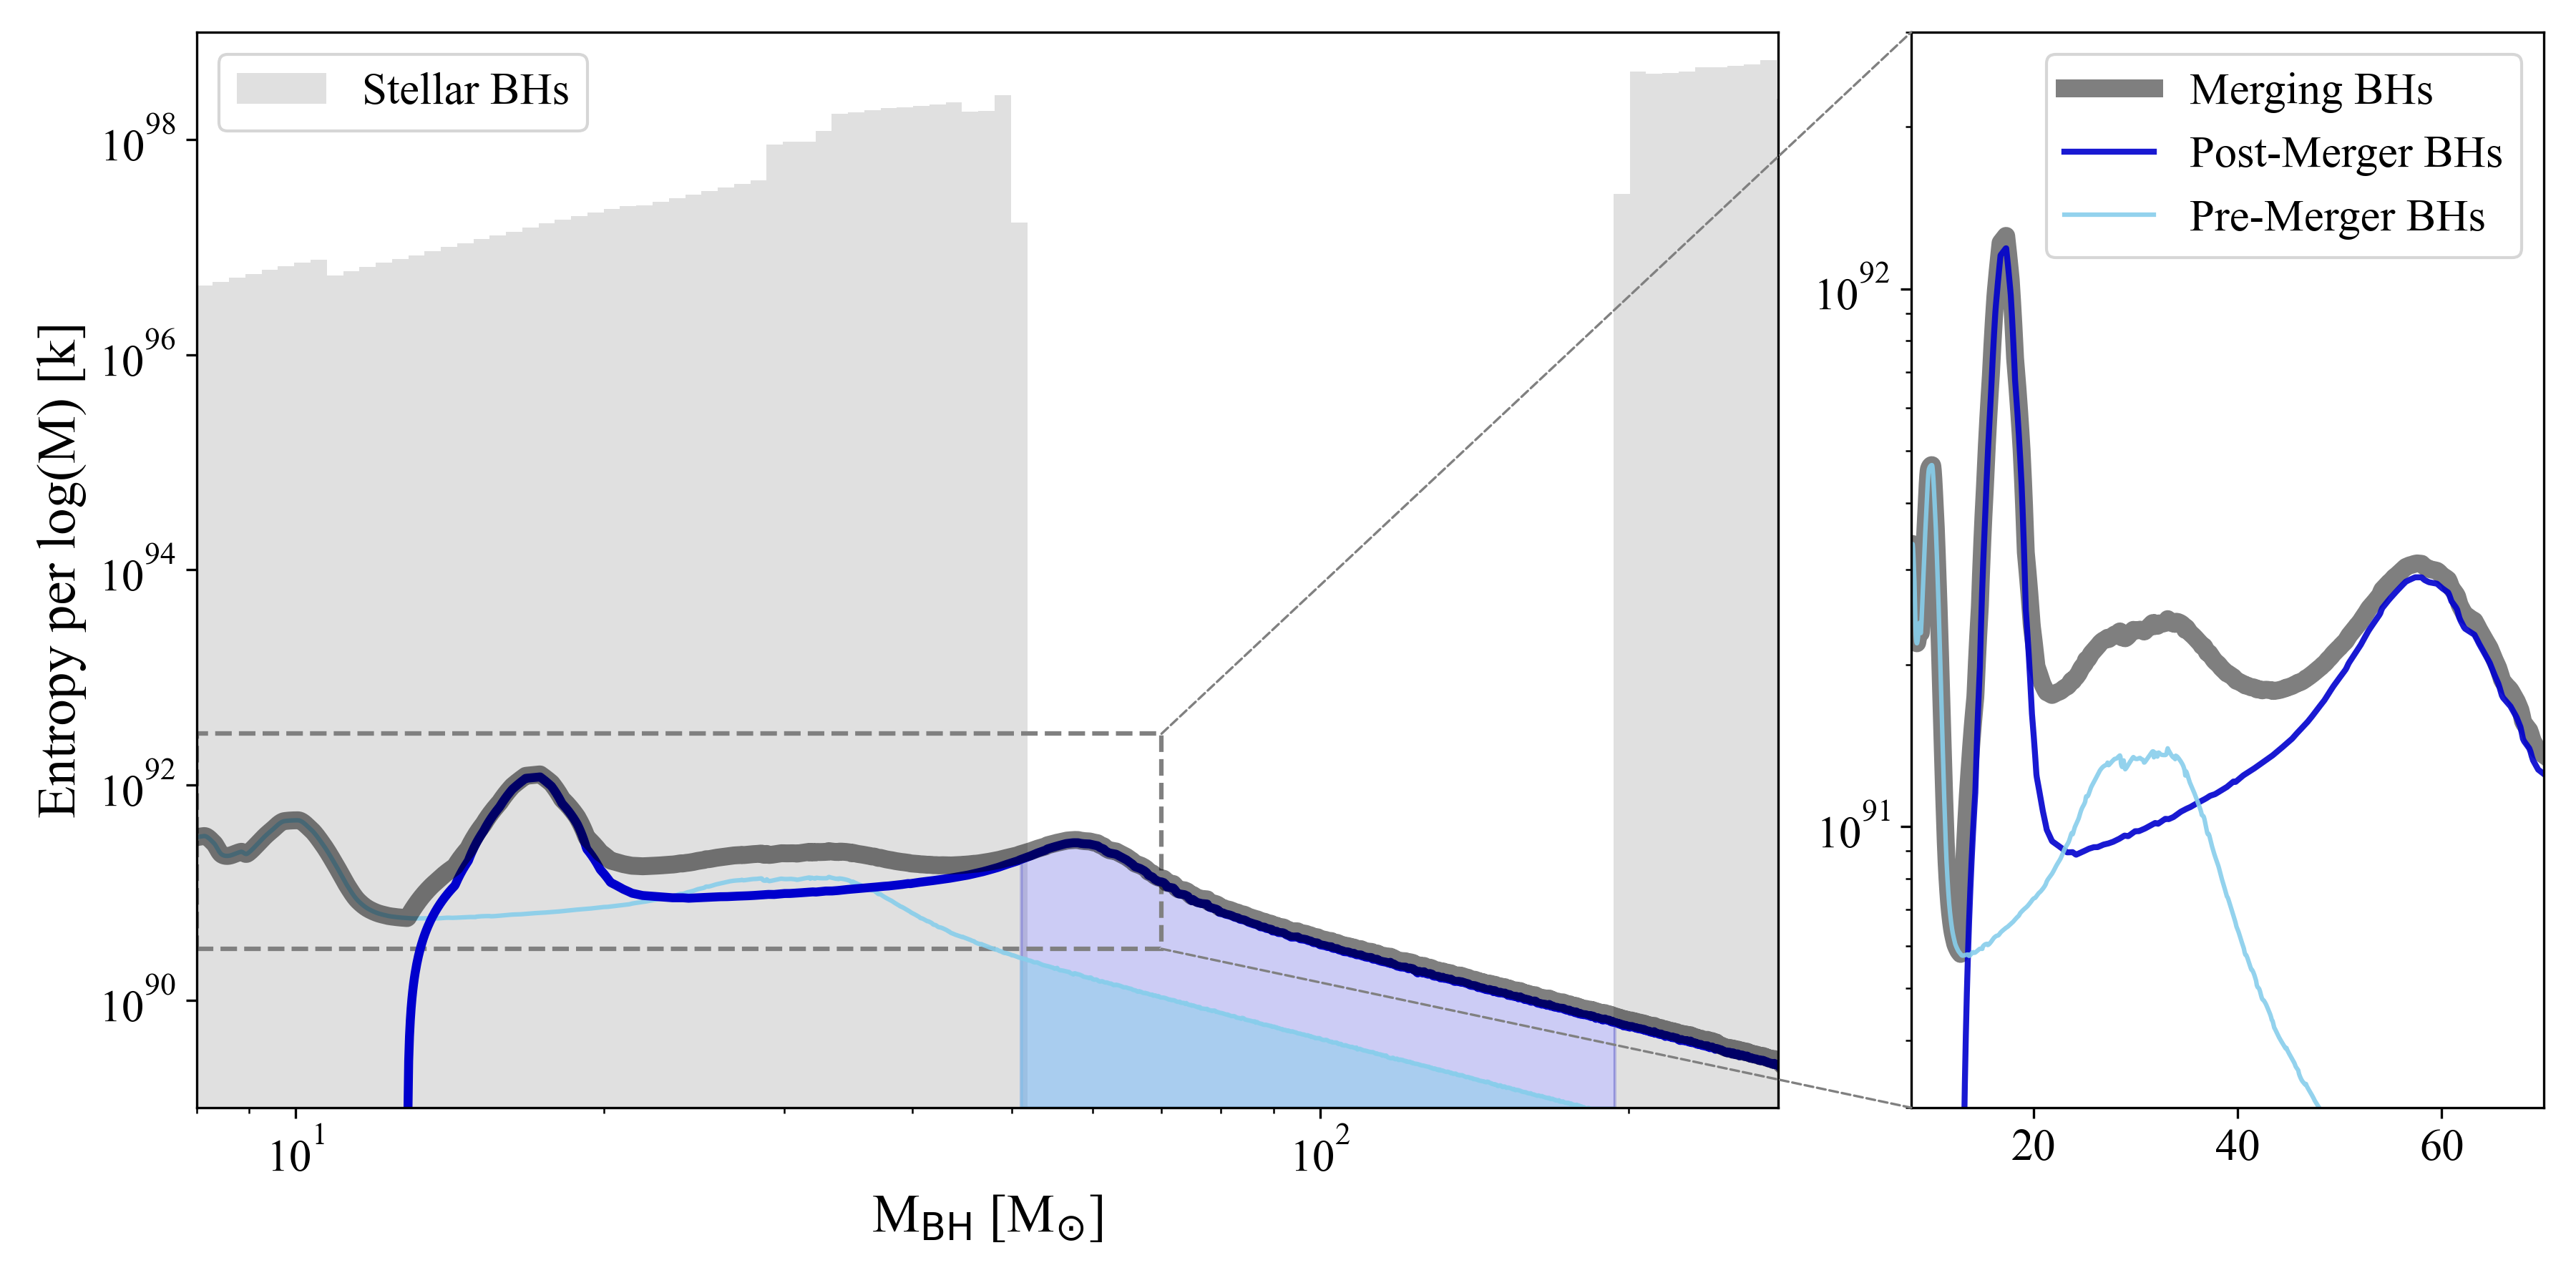
\includegraphics[trim = 0 10 0 0, clip, width=0.98\textwidth]{pisn_bh_imf_gwtc4.png}
\caption{\textbf{Cosmological Binary Black Hole Entropy Inventory}: the total accumulated entropy (Static Budget) from different black hole populations as a function of black hole mass. The stellar–origin black holes (grey histogram) include black holes formed via supernova and direct collapse. The population of merging black holes is decomposed into pre-merger components (light blue) and post-merger remnants (dark blue), both contributing in the range $5-200~M_\odot$. The total entropy budget from merging binaries is shown as a thick gray band. The right panel zooms in on the entropy profile of merging black holes in the range $8-70~M_\odot$ to highlight the detailed structure.}
%The left axis and the blue  bins show the number density per log(M) for black holes inferred from the Salpeter IMF and the mass distribution of remnant black holes from \cite{Spera_2017}. The right axis and the red curves show the entropy of black holes per log(M). Three different red curves represent three different black hole categories.}
\label{fig:imf}
\end{figure*}

In this study, we categorize stellar-origin black holes (remnants of stellar collapse) into three specific regimes. We define standard \textit{stellar BHs} as having $5 -45~M_\odot$. Objects residing within the PISN mass gap, $45-130~M_\odot$, are referred to as \textit{PISN BHs}. Very massive stars (VMS, $\gtrsim 260~M_\odot$) may instead collapse directly, bypassing the PISN mechanism and producing remnants in the range of $130-300~M_\odot$, which we denote as \textit{lite-IMBHs} \citep{Woosley_2017, Ezquiaga_2021, Mehta_2022, franciolini2024farsideobservingblack, Ruiz-Rocha2025yno, Chatterjee_2025}. More broadly, we adopt $10^2 - 10^7~M_\odot$ as the \textit{IMBHs} range. Finally, black holes exceeding $10^7~M_\odot$ are classified as supermassive black holes (\textit{SMBHs}). Although rare in number, SMBHs are expected to be the dominant contributors to the total cosmic entropy budget. All entropies are expressed in units of $k$ and compared on a common comoving basis.

To compute the total number density of massive stars that can collapse into black holes, we adopt the Salpeter Initial Mass Function \citep[IMF;][]{1955ApJ...121..161S} parameterized by a power-law index $\alpha = 2.35^{+0.35}_{-0.65}$:

\begin{equation}
\xi(m_\star)~dm = \xi_0 \left( \frac{m_\star}{M_\odot} \right)^{-\alpha} dm,
\end{equation}
where $\xi_0$ is the normalization constant. We calibrate $\xi_0$ by requiring that the integral of the mass-weighted IMF over the full stellar mass range (assumed to be $0.1 - 350\,M_\odot$) reproduces the observed present-day cosmic stellar mass density, $\Omega_\star \simeq 0.0027\pm0.0005$ \citep{Fukugita_2004, Madau_2014}:

\begin{equation}
  \rho_\star = \int^{350~M_\odot}_{0.1~M_\odot} m_\star\,\xi(m_\star)\,dm_\star = \Omega_\star\,\rho_{\rm c,0}
\end{equation}
where $\rho_{\rm c,0}$ is the critical density of the universe at $z=0$, assuming a flat $\Lambda$CDM cosmology \citep{2020A&A...641A...6P}.

With $\xi_0$ determined, the number density of black hole progenitors within the specific mass interval $[m_{\rm min}, m_{\rm max}] = [8, 350]\,M_\odot$ is given by:
\begin{equation}
    n_\star = \int^{m_\mathrm{max}}_{m_\mathrm{min}} \xi(m_\star)~dm_\star
    \label{eq:numberimfstars}
\end{equation}

For each progenitor mass $m_\star$, we determine the corresponding remnant mass, $m_{\rm rem}$, using the SEVN stellar evolution code \citep{Spera_2017}. We assume a low-metallicity environment ($Z=2\times10^{-4}$) to account for the formation of massive black holes and include the effects of PPISN and PISN.

We note that the mapping $m_\star \mapsto m_{\rm rem}$ is non-bijective due to mass-loss pile-ups (PPISN) and complete disruptions (PISN). Consequently, a simple Jacobian transformation of the IMF is invalid \citep{Jani_2020}. Instead, we compute the remnant mass function, $\xi_{\rm BH}(m_{\rm rem})$, by enforcing particle number conservation: we sum the IMF contributions from all disjoint progenitor intervals that map into a given remnant mass bin.

To determine the total number density of black holes and their cumulative contribution to the cosmic entropy budget, we integrate the derived remnant mass function, $\xi_{\rm BH}(m_{\rm rem})$, over the remnant mass range. For the entropy calculation, we require a spin assignment for each black hole. We assume a uniform distribution for the dimensionless spin parameter, $a \sim \mathcal{U}[0,1]$, and compute the entropy for each remnant mass using Eq. \ref{eq:entropy}. The resulting distributions of remnant count and total entropy are illustrated by grey histograms in Fig. \ref{fig:imf}.

\begin{comment}
    
The total number of massive stars that can collapse into black holes \citep{Jani_2020} can be calculated by:

\begin{equation}
    N_s = \psi(z) \times n_s~[Mpc^{-3}~yr^{-1}]
\end{equation}
% Salpeter IMF $\xi(m)$:

where $\psi(z)$ is the star formation rate measured from  far-UV and far-infrared \citep{Madau_2014}:
\begin{equation}
    \psi(z) = 0.015 \times \frac{(1+z)^{2.7}}{1+(\frac{1+z}{2.9})^{5.6}} ~[M_\odot~Mpc^{-3}~ yr^{-1}]
\end{equation}

% Since we are working in terms of mass, we integrate $\psi(z)$ across the redshift range to compute the number of stars in the observable universe.

Since our analysis is conducted in terms of mass, we integrate $\psi(z)$ over the relevant redshift range to estimate the total number of stars for each mass interval in the observable universe.

$n_s$ is defined as the number of progenitor stars that can collapse as black holes per unit mass, which can be computed by:

\begin{equation}
    n_s = \frac{\int^{m_\mathrm{max}}_{m_\mathrm{min}}\xi(m)~dm}{\int^{1000~M_\odot}_{0.01~M_\odot}m~\xi(m)~dm}~[M_\odot^{-1}]
\end{equation}

Here $\xi(m)~dm$ represents the initial mass function (IMF), which describes the mass distribution of stellar formation. In this study, we adopt the Salpeter IMF \citep{1955ApJ...121..161S, Egan_2010} with $\alpha = -2.35^{+0.65}_{-0.35}$:

\begin{equation}
    \frac{d\xi (M)}{d log(M)} \propto (\frac{M}{M_\odot})^{\alpha+1}
\end{equation}


By definition of IMF, we can compute the total number of stars N within the mass interval $[m_\mathrm{min}, m_\mathrm{max}]$ by integrating:
\begin{equation}
    N = \int^{m_\mathrm{max}}_{m_\mathrm{min}} \xi(m)~dm
    \label{eq:numberimfstars}
\end{equation}

In this study, we define the mass bounds $m_\mathrm{min} = 8~M_\odot$ and $m_\mathrm{max} = 350~M_\odot$, which is consistent with the $M_\mathrm{ZAMS}$ range listed in \cite{Spera_2017}. Then, we can derive a normalization factor $\xi_0$:

\begin{equation}
    \xi_0 = \frac{N_s}{N}
\end{equation}

The IMF at each $m_\mathrm{star}$ is thus:
\begin{equation}
    \xi(m_\mathrm{star})~dm = \xi_0~(\frac{m_\mathrm{star}}{M_\odot})^{-2.35} ~(\frac{dm}{M_\odot})
\end{equation}

\end{comment}

% We determine the mass of the remnant compact object, $m_\mathrm{rem}$, that forms from a progenitor star of initial mass $m_\mathrm{star}$ by utilizing the stellar evolution and remnant mass prescription provided in \cite{Spera_2017}. We assume low stellar metallicity $Z = 2 \times 10^{-4}$ and account for the PISN effect. Since the mapping between $m_\mathrm{star}$ and $m_\mathrm{rem}$ is not bijective, we compute the IMF $\xi(m_\mathrm{rem})~dm$ by summing the contributions of $\xi(m)~dm$ from all progenitor masses that correspond to the same $m_\mathrm{rem}$ \citep{Jani_2020}.
% \scccc{Let's define somewhere at the start what is the mass-range of stellar BH (5-45), PISN BHs (45-120), lite-IMBH (120-500) etc.   }
% Stellar black holes ($1.3 - 44.8~M_\odot$) originate from progenitor stars in the range $8-111.5~M_\odot$, while IMBHs from VMSs ($197.4 - 281.2~M_\odot$) form from progenitors with masses between $232.2 - 350~M_\odot$ \citep{Spera_2017}. 
% To compute the total number of objects in each black hole category - and subsequently their contribution to the entropy budget - we integrate $\xi(m_\mathrm{rem})~dm$ using Eq. \ref{eq:numberimfstars} within the corresponding mass bounds \footnote{The upper and lower mass bounds for stellar BHs and light-IMBHs come from the results in \cite{Spera_2017}.}.

% With the number of black holes for each mass $m_\mathrm{rem}$, we compute the entropy for 

% After obtaining the number of black holes for each mass $m_\mathrm{rem}$, we uniformly sample the spin magnitude $a$ from the range $[0,1]$ and compute the total entropy of black holes with $m_\mathrm{rem}$ using Eq. \ref{eq:entropy}. These entropies are visualized in green and orange bars in Fig. \ref{fig:imf}.
%\scccc{for individual BHs we should assume uniform distribution of spin from 0 to 1. For merging BBH, we use GWTC}

% \scccc{Karan - how do you get entropy of stellar BHs from this equation? Write it down. }

\subsection{Entropy for Merging Binary Black Holes}

For merging BBHs, we can get 4 different types of entropies: entropy of the primary black hole ($S_1$), entropy of the secondary black hole ($S_2$), entropy of the remnant black hole ($S_\mathrm{f}$), and the entropy produced during the merger ($\Delta S$), which can be calculated by:

\begin{equation}
\label{eq:delta-entropy}
\centering
    \Delta S = S_\mathrm{f} - (S_1 + S_2)
\end{equation}

% In this study, we will also use $S_1$, $S_2$, and $S_\mathrm{f}$ from merging BBHs to compute the entropy of individual black hole populations.

To compute the entropy change for individual BBHs reported by LVK, we utilize the parameter estimation results made available in the GW Open Science Center \citep{2021SoftX..1300658A, 2023ApJS..267...29A}. We adopt posterior samples obtained with the IMRPhenomXPHM waveform model \citep{Khan_2016, Khan_2019, Pratten_2020, Pratten_2021, dambrosio2024testinggravitationalwaveformsgeneral}. These samples include the mass and spin associated with the corresponding remnant black hole, which has been computed using phenomenological fits to numerical relativity (NR) results \citep{Santamar_a_2010, Hofmann_2016, Healy_2017, Jim_nez_Forteza_2017,  Estell_s_2022}. For each posterior sample, we evaluate Eq. \ref{eq:entropy} for the primary, secondary, and remnant black holes to obtain ($S_1, S_2, S_\mathrm{f}$) and then compute the entropy change $\Delta S$ with Eq. \ref{eq:delta-entropy}. The resulting event-level $\Delta S$ measurements are summarized in Fig. \ref{fig:lvk}.

\begin{figure}[hbt!]
\centering
% \includegraphics[width=0.49\textwidth]{mass-entropy.png}
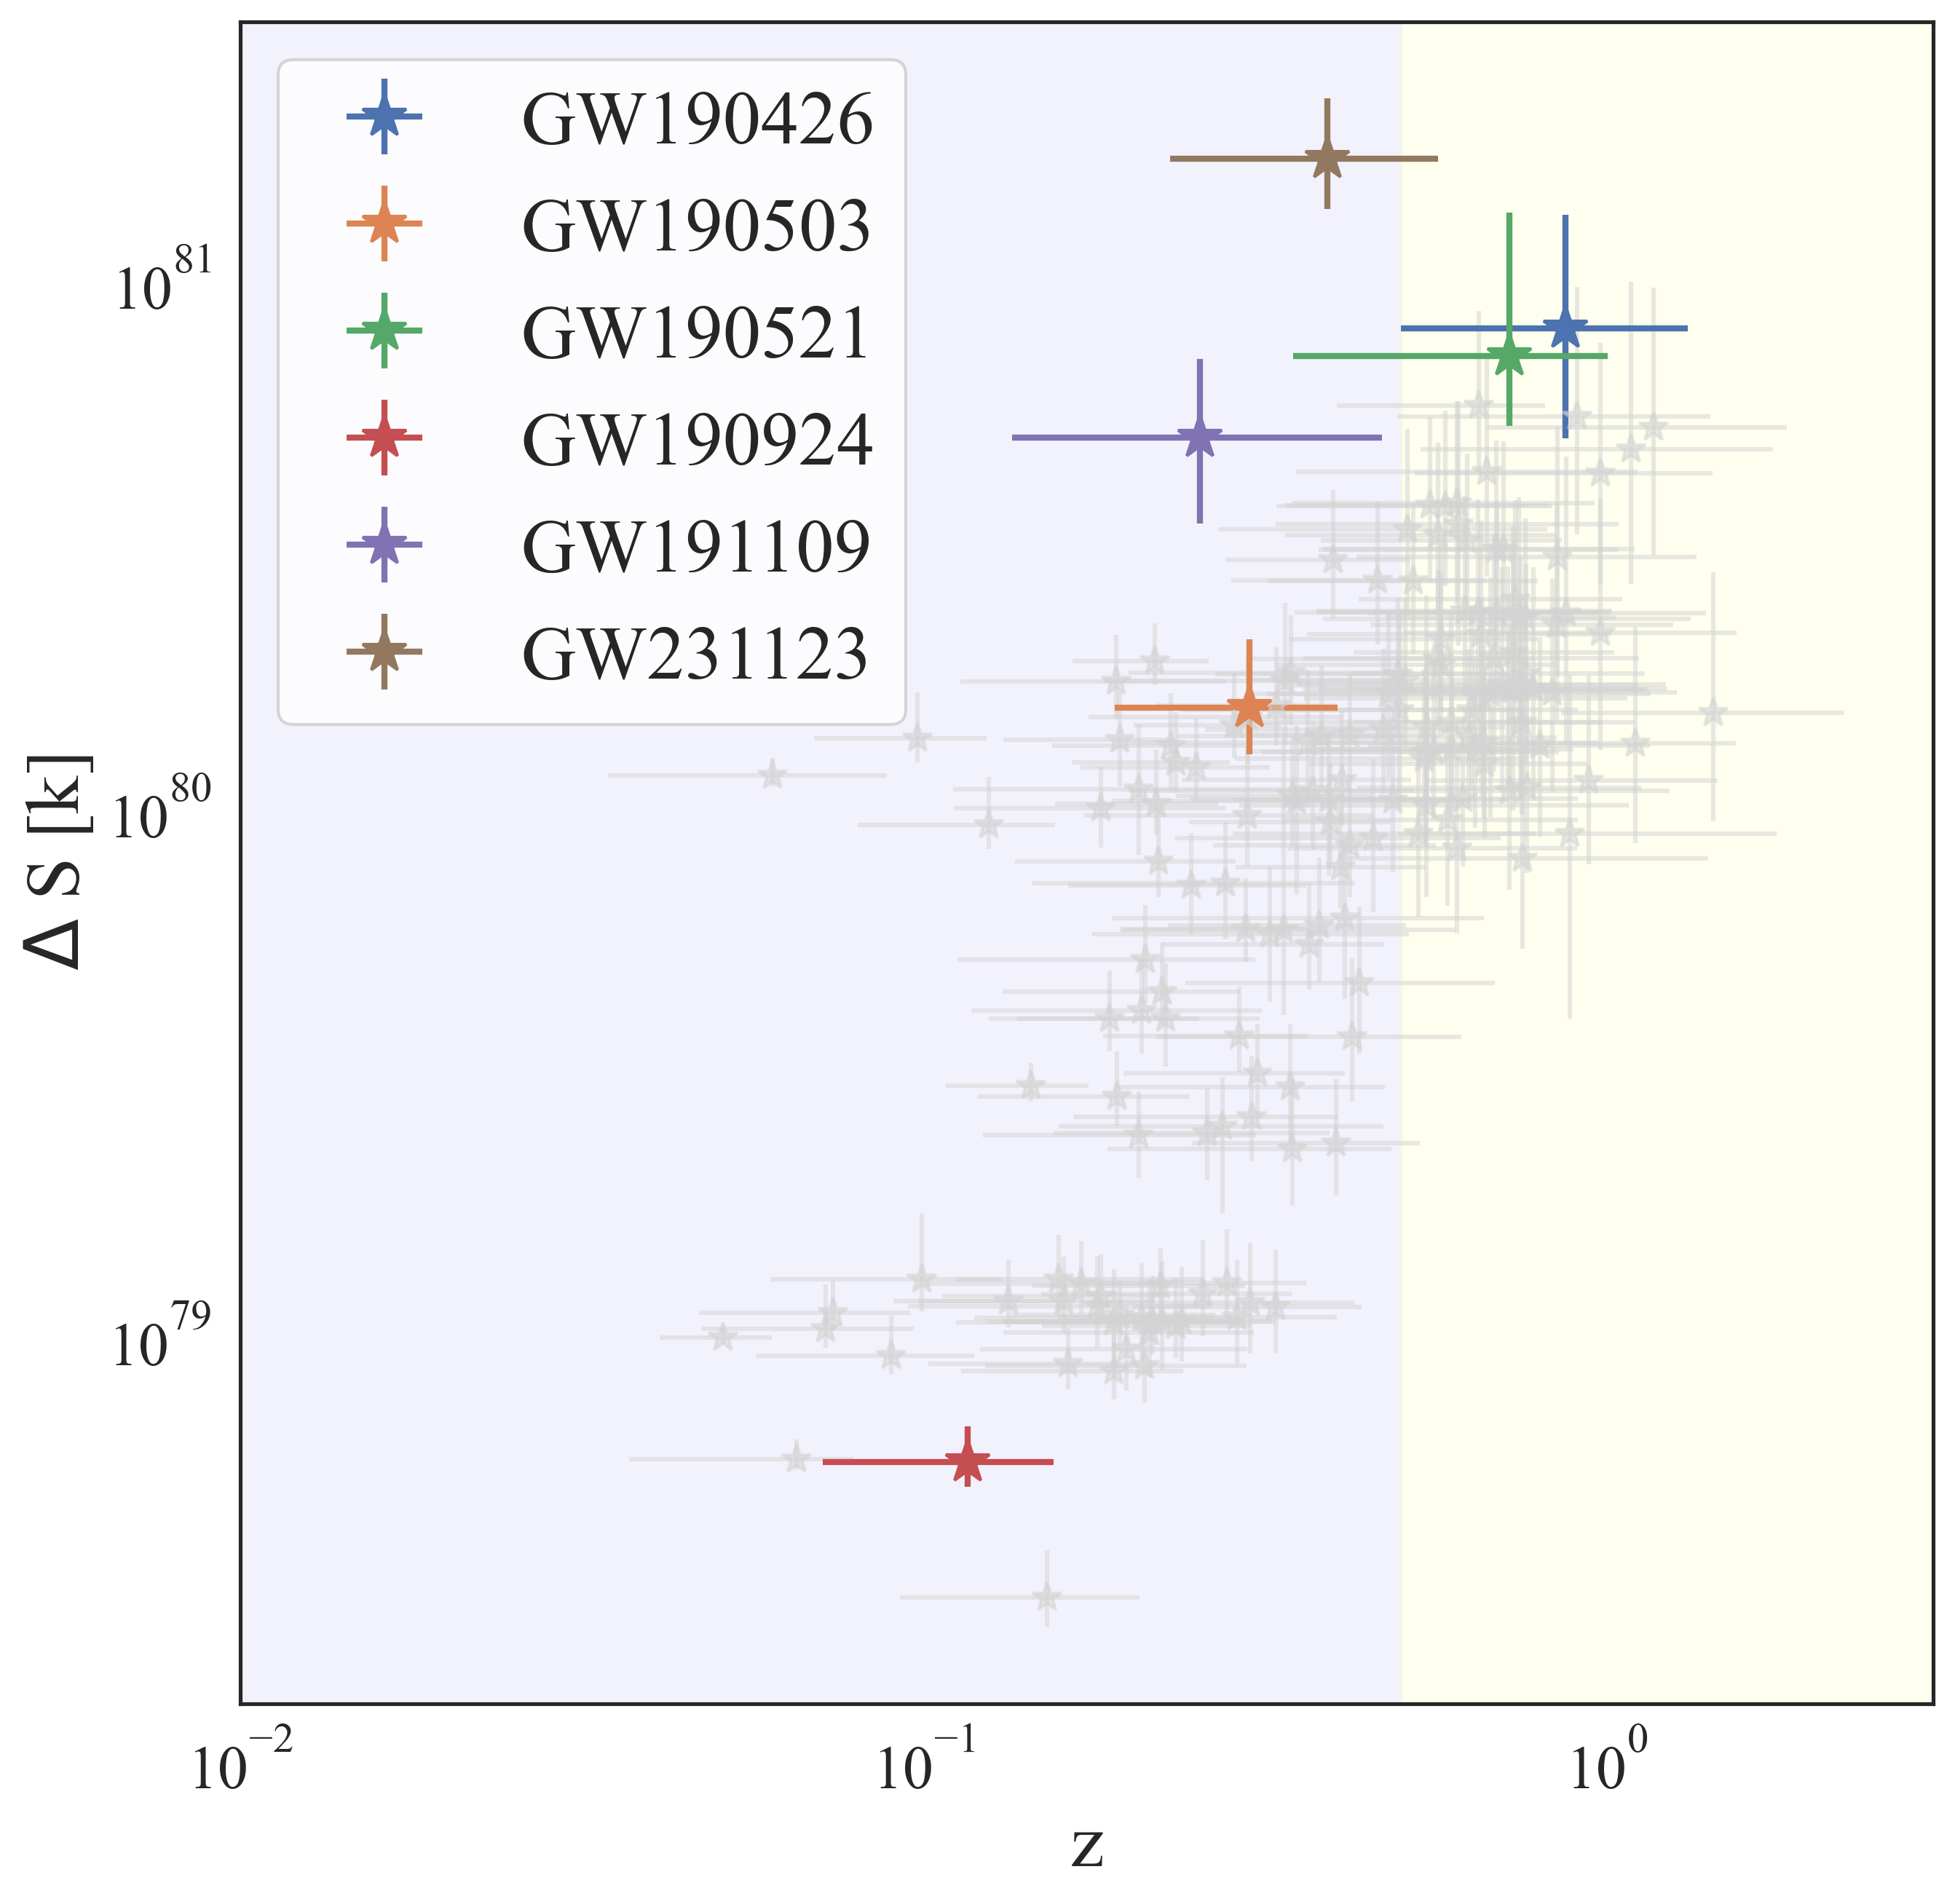
\includegraphics[width=0.49\textwidth]{redshift-entropy.png}
\caption{\textbf{Entropy Production in Individual GW Events}: grey bars show the correlation between the redshift of the binary and the change in entropy during BBH mergers for 168 BBH events reported by LVK. The bar represents $z$ and $\Delta~S$ with 90\% confidence interval. Certain GW events are highlighted in color. The purple-shaded region corresponds to the dark energy–dominated era ($z \le 0.5$), while the yellow-shaded region represents the matter-dominated era ($z > 0.5$).}
\label{fig:lvk}
\end{figure}

To extend the analysis to the population level, we adopt the Power Law + Peak (PP) model \citep{Talbot_2018}, which demonstrates the highest Bayes factor in characterizing the Gravitational-Wave Transient Catalog dataset of the Third / Fourth Observing Run (GWTC-3 / 4). The detailed parameter distributions are described in \cite{gwtc-3-pop, gwtc4pop}. To propagate population-level uncertainties into our entropy estimates, we evaluate results using representative lower and upper bounds of the BBH merger rate inferred by LVK (as reported in the catalog analyses). This brackets the range of plausible merger-driven entropy production within the model and catalog uncertainties.

Given the hyperparameterized distributions of the PP model, we generate a Monte Carlo sample of $N_\mathrm{BBH}$ synthetic binaries by drawing inspiral parameters $\Lambda^\mathrm{ins}_i: \{ m_{1,2},~a_{1,2},~\theta_{1,2} \}$ with bounds determined by the adopted population model. For each draw $\Lambda^\mathrm{ins}_i$, we compute the remnant parameters $\Lambda^\mathrm{rem}_i: \{ m_\mathrm{f},~a_\mathrm{f} \}$ using the NR surrogate fit \textsc{NRSur7dq4Remnant} \citep{Blackman_2017, Boschini_2023} as implemented in the \textit{SurfinBH} package \citep{soft09007V, Varma_2019, zertuche2024highprecisionringdownsurrogatemodel}. We then evaluate Eq. \ref{eq:entropy} to obtain ($S_1, S_2, S_\mathrm{f}$) and Eq. \ref{eq:delta-entropy} to compute the corresponding entropy change $\Delta S$.

% From the parameter distributions of PowerLaw + Peak model, we resampled $N_\mathrm{BBH}$ individual binaries with Monte Carlo sampling for inspiral parameters $\Lambda^\mathrm{ins}_i: \{ m_{1,2},~a_{1,2},~\theta_{1,2} \}$. The bounds on $\Lambda^\mathrm{ins}_i$ are dictated by the population. To obtain the corresponding parameters of the remnant black hole, $\Lambda^\mathrm{rem}_i: \{ m_\mathrm{f},~a_\mathrm{f} \}$, we utilize the phenomenological fit \textsc{NRSur7dq4Remnant} \citep{Blackman_2017, Boschini_2023} from the \textit{SurfinBH} package \citep{soft09007V, Varma_2019, zertuche2024highprecisionringdownsurrogatemodel}. For each $\Lambda_i$, we compute $S_i$ using Eq. \ref{eq:entropy}. 
%The sample size is the total number of BBH mergers $N_\mathrm{BBH}$.


% To sample inspiral parameters $\theta(m_1, q, a_1, a_2, \theta_1, \theta_2, z)$, we adopt the Power Law + Peak model \citep{Talbot_2018}, which demonstrates the highest Bayes factor in characterizing GWTC-3 populations. This model assumes independent and uncorrelated spin and mass distributions. The most notable feature for this model is the small peak at $\sim 35~M_\odot$ in the primary mass distribution due to the PISN mass gap \citep{Farmer_2019, Farmerconstra_2020, Edelman_2022, gwtc-3-pop}. For computational simplicity, the model assumes $\chi_{1}$ = $\chi_{2}$ and a uniform distribution for inclination angle across [0, $\pi$]. We obtain the individual inspiral parameter $\theta_i$ from its corresponding hyperposterior sample by reverse CDF sampling. We drew a large number of 



% The model assumes that spin and mass are independent and uncorrelated. Therefore, the hyperposterior gives different distributions to describe $m_{1}$, $m_{2}$ (mass), $\chi_{1}$, $\chi_{2}$ (spin magnitude), and z (redshift). 


% For computational simplicity, we assume that $a_{1}$ = $a_{2}$. The spin of primary and secondary black holes also display similar posteriors, so the assumption will not exert a large effect. By implementing the reverse CDF (cumulative distribution function) sampling and rejection sampling, we draw individual merger samples from the distributions derived from gravitational wave observations. These mergers are binary black hole mergers with masses between [2.5, 100]$M_{\odot}$ in the source frame and spin between [0, 1]. We assume these mergers happen within $z \le 1.5$. The population modeling gives us robust measurements of the pre-merger binary black holes, which enables us to calculate the initial entropy.



% LIGO can estimate the merger rate from existing BBH detection. We adopt the merger rate inferred from GWTC-3 (Gravitational Wave Transient Catalog) \citep{gwtc-3}. At z=0.2, the BBH merger rate is inferred to be [17.9, 44] GPc$^{-3}$yr$^{-1}$ \citep{KAGRA:2021duu}. Due to a large number of BBH detections, the range for the BBH merger rate is relatively small. Therefore, we can accurately estimate the total number of BBH populations in the universe, further calculating the total entropy change $\Delta$S from BBH mergers. 

% To compute the entropy density in the universe, we will need to calculate the volume of the universe. However, the universe is expanding, so cosmological distance will change over time, which makes it difficult to compute the volume of the universe. Therefore, we adopt the notion of the ``comoving coordinates," which scales with the expansion of the universe. The calculated comoving volume will be independent of the expansion. To compute such volume, we first need to calculate the comoving distance:

% \begin{equation}
% \centering
% l_{c} = \int_{z_{1}}^{z{2}} \ddfrac{c} {H_{0} \sqrt{\Omega_{M}(1+z)^3 + \Omega_{\Lambda}}}\mathrm{d}x
% \end{equation}

% where cosmological constants $\Omega_{M}$ = 0.3 represents the density of matter (normal \& dark matter) and $\Omega_{\Lambda}$ = 0.7 represents the density of energy in the universe. We utilize the value $H_{0}$ = 70 $\mathrm{km s^{-1}MPc^{-1}}$ for Hubble constant measured from GW170817 \citep{2017}. For simplicity, we assume that the observable universe is spherical, we can calculate the comoving volume by 

% \begin{equation}
% \centering
%     V_{c} = \frac{4}{3} \pi l_{c} ^ 3
% \end{equation}

% The entropy density at redshift z can be computed as $\frac{S}{V_{c}}$, with a lower bound of z and upper bound of $\infty$ plugged in the comoving distance integral. We can also use functions from the astropy package to help.

% Gravitational wave detectors are not perfect and obtain selection effects. GW sources are more likely to come from certain sky localization or certain times during the duty cycle. The sensitivity regions for the two LIGO detectors are above North America and the Indian Ocean. As the Earth rotates, the regions will swipe the entire sky localization. Meanwhile, the detectors have the preference to collect data at night \citep{2017ApJ...835...31C}. As a result, GW detectors tended to detect black holes with certain masses due to the sensitivity range that targets specific frequencies. As discussed in Section \ref{sec:intro}, entropy largely depends on the mass, so we need to correct these biases when constructing the entropy distribution for compact object populations. We perform population analyses to infer the pre- and post-merger conditions of BBH mergers. 


% \subsection{Population Modeling \& Sampling}


% \begin{equation}
% \centering
% N = zppd \times V_{c} \times t = \mathrm{zppd} \times \frac{4}{3}\pi (l_{c} \times 10^{-3}) ^ 3 \times t
% \label{eq:merger}
% \end{equation}

% We denote zppd as the merger rate associated with redshift $z_{2}$. $l_{c}$ is calculated in terms of MPc from $H_{0}$, so we use a factor of $10^{-3}$ to match the GPc used in Power Law + Peak model. We use the astropy package with Planck18 cosmology to figure out the age (t) at a particular redshift.


% \subsection{Surrogate Final Black Hole Properties}
%  To get the remnant population $\theta^\mathrm{rem}_i$, we adopt numerical relativity, which solves Einstein's equations of general relativity \citep{PhysRevLett.95.121101, PhysRevLett.96.111101, PhysRevLett.96.111102, Palenzuela_2020} and numerically fits the quasinormal mode to the post-merger black hole \citep{Buonanno_2007, Berti_2007,hengrui_2024, Gennari_2024}. We use the \textbf{NRSur7dq4Remnant} surrogate model from \textit{SurfinBH} package  %(\textbf{Sur}rogate \textbf{fin}al \textbf{B}lack \textbf{H}ole) 
% \citep{soft09007V, Varma_2019, zertuche2024highprecisionringdownsurrogatemodel}, which estimates the properties of the remnant black hole based on the inspiral parameters $\theta_{i}(m_i, \chi_i, \iota_i)$. The algorithm derives the post-merger mass, spin, and kick velocity, giving us the post-merger parameters to compute $\mathcal{I}_\mathrm{BBH}$ with entropy of the remnant black hole. With $\theta_i$ and $\theta^\mathrm{rem}_i$, we can calculate $S_\mathrm{f}, S_1, S_2$ of each BBH merger sample, thus computing the $\mathcal{I}_\mathrm{BBH}$ posterior.


% Numerical relativity solves Einstein's equations of general relativity, which characterizes the gravitational wavelet. Previously, we have shown that the NRSur7dq4 waveform gives the highest consistency in our IMR consistency test. Similarly, we utilize the \textbf{NRSur7dq4Remnant} fit from the SurfinBH (\textbf{Su}rrogate \textbf{fin}al \textbf{B}lack \textbf{H}ole) package \citep{Varma_2019}. This package estimates the properties of the remnant black holes. Inferred from the input pre-merger parameters, the package approximates the final mass, spin, and recoil kick velocity. With the mass and spin estimated, we can calculate the final entropy. 

% \begin{figure}[hbt!]
% \centering
% \includegraphics[width=0.6\textwidth]{surfinbh.png}
% \caption{BBH merger mechanism with GWs radiate to spacetime. SurfinBH package helps to infer $m_f$, $\chi_f$, and $v_f$ from the pre-merger parameters $m_{1,2}$, $\chi_{1,2}$ through numerical relativity fitting.}
% \label{fig:surfinbh}
% \index{figures}
% \end{figure}

% With the pre-merger entropy calculated from Power Law + Peak and the post-merger entropy calculated from the SurfinBH package, we can compute the increase in total entropy from BBH mergers and the difference in entropy density. Together with the distributions that characterize the GWTC-3 dataset, we model the correlation between entropy and other parameters, including redshift.

% \subsection{Merger Rates Calculation}
\label{subsec:mergerrate}
Observational constraints from GWTC-3/4 population analyses parameterize the BBH merger-rate density as a redshift-dependent power law $\mathcal{R}_\mathrm{BBH}(z) \propto (1+z)^\kappa$ \citep{gwtc-3-pop, gwtc4pop}. Owing to the sensitivity of current ground-based detectors, this evolution is directly constrained primarily in the local universe, roughly over $z \in [0.2, 1.5]$. For $z \ge 1.5$, we utilize $\mathcal{R}_\mathrm{BBH}(z)$ reported in \cite{Mapelli_2018} derived from the Illustris simulation. In this work, we discretize redshift into bins uniform in lookback time with $\Delta t_\mathrm{lb}= 10^7~yr$. 

The merger rate may be written as $\mathcal{R}(z) = dN_\mathrm{BBH}/(dV_c~dt)$ \citep{Mandel_2022, gwtc-3-pop}. The expected number of BBH mergers in a lookback-time bin centered at redshift $z$ is then
\begin{equation}
    \centering
    \label{eq:growth}
    N_\mathrm{BBH}(z) = \mathcal{R}(z) \times \Delta V_c(z) \times \Delta t_\mathrm{lb}(z)
\end{equation}
where $\Delta V_c$ is the differential comoving volume element associated with the bin and $\Delta t_\mathrm{lb}$ is the corresponding lookback-time width. For each bin, we draw $N_\mathrm{BBH}(z)$ sets of inspiral parameters $\Lambda^\mathrm{ins}_i$ from the adopted population model and compute the corresponding entropy changes $\Delta S_i$. The total merger-generated entropy in that bin is therefore $\sum_{i=1}^{N_\mathrm{BBH}} \Delta S_i$. \footnote{For computational efficiency, we only sample and compute the total entropy change of $10^6$ mergers and scale with $N_\mathrm{BBH}$.}

We also consider the corresponding entropy density, defined as
\begin{equation}
    \centering
    s = \frac{S}{V_\mathrm{obs}}
    \label{eq:density}
\end{equation}
where $V_\mathrm{obs}$ is the volume of the observable universe. We adopt $3.52^{+0.11}_{-0.11} \times 10^{80}~m^3$ \citep{profumo2024newcensusuniversesentropy}. %The resulting redshift evolution of the total entropy and entropy density from BBH mergers is shown in Fig. \ref{fig:growth}.

\begin{table*}[t!]
\caption{Updated entropy budget table of different cosmological components in the observable universe, with comparisons to previous work. The IMBH category remains poorly constrained observationally, leading to large uncertainties in entropy estimates. All entropy densities computed by dividing by $V_\mathrm{obs}$. Reference: 
[1] \cite{Frautschi1982}, 
[2] \cite{Frampton_2008},
[3] \cite{frampton2009entropyintermediatemassblackholes},
[4] \cite{Frampton_2009},
[5] \cite{Egan_2010},
[6] \cite{profumo2024newcensusuniversesentropy}
}

\label{tab:budget}

\resizebox{\textwidth}{!}{%
\begin{tabular}{llll}
\hline\hline
\textbf{Components} & \textbf{Entropy Density $s$ [$k~\mathrm{m}^{-3}$]} & \textbf{Entropy $S$ [$k$]} \ \ \ \ & \textbf{Entropy $S$ [$k$] } \\
 &   & \textbf{(This Work)} & \textbf{(Previous Work)} \\
\hline 
Stellar BHs ($5{-}45~M_\odot$) & $1.8 \times 10^{18^{+0.8}_{-2.1}}$ & $2.8 \times 10^{98^{+0.8}_{-2.1}}$ & $10^{96}$ [6], $10^{97}$ [4][5], $10^{98}$ [1] \\

PISN BHs ($45{-}130~M_\odot$) & $1.2^{+1.3}_{-0.5} \times 10^{12}$ & $1.9^{+2.1}_{-0.7} \times 10^{93}$ & $10^{99}$ [5]\\

Lite-IMBHs ($130{-}300~M_\odot$) & $5.1 \times 10^{18^{+0.9}_{-1.6}}$ & $1.8 \times 10^{99^{+0.9}_{-1.6}}$ & - \\

IMBHs ($10^2{-}10^7~M_\odot$) & $1.4 \times 10^{17^{+8.3}_{-1.2}}$ [3][6] & - &  $10^{97}$ [6], $10^{105}$ [3] \\
SMBHs ($10^7{-}10^9~M_\odot$) & $2.4^{+3.0}_{-2.2} \times 10^{21}$ [6] & - & $10^{101}$ [6], $10^{102}$ [4], $10^{103}$ [2], $10^{104}$ [5]\\

\hline
BBH mergers $\Delta S$ ($5{-}\sim 500~M_\odot$) & $7.1^{+9.2}_{-3.5} \times 10^{12}$ & $1.1^{+1.5}_{-0.6} \times 10^{93}$ & - \\
GWTC Pre-merger $S$ ($5{-}300~M_\odot$) & $1.2^{+1.5}_{-0.6} \times 10^{13}$ & $1.9^{+2.5}_{-0.9} \times 10^{93}$ & - \\
GWTC Post-merger BHs ($8{-}\sim 500~M_\odot$) & $1.9^{+2.5}_{-0.9} \times 10^{13}$ & $3.1^{+4.0}_{-1.5} \times 10^{93}$ & - \\

\hline
Photons & $1.5 \times 10^{9}$ [6] & - & $10^{88}$ [4], $10^{89}$ [5][6]\\
Relic Neutrinos & $1.4 \times 10^{9}$ [6] & - & $10^{88}$ [4], $10^{89}$ [5][6]\\
WIMP Dark Matter & $8.9^{+64}_{-6.0} \times 10^{7}$ [6] & - & $10^{88}$[5], $10^{87}{-}10^{89}$[6]\\
Relic Gravitons & $1.7 \times 10^{{7}^{+3.5}_{-2.5}}$ [5][6] & - & $10^{87}$ [5], $10^{87}{-}10^{91}$[6]\\
ISM and IGM & $7.5^{+1.1}_{-7.0} \times 10^1$ [5][6] & - & $10^{81}$[5], $10^{80}{-}10^{81}$[6]\\
Stars & $2.6\times10^{{-1}^{+4.5}_{-3.7}}$ [5][6] & - & $10^{79}$ [4],$10^{80}$ [5], $10^{74}{-}10^{81}$[6]\\
\hline\hline
\end{tabular}%
}
\end{table*}



% \scccc{Explain that we get four entropies from merging BBH: primary m1, secondary m2, remnant mf and entropy released. We will use m1, m2 and mf to populate entropy from stand alone BHs}

\subsection{Entropy Budget for Primordial Black Holes}
To contextualize the entropy contribution of stellar-origin black holes, we consider the potential contribution from PBHs. PBHs are hypothetical compact objects formed in the radiation-dominated era ($z \gtrsim 3000$), which may constitute a fraction $f_\mathrm{PBH} \equiv \Omega_\mathrm{PBH} / \Omega_\mathrm{DM}$ of the total dark matter density, where $\Omega_\mathrm{DM} \approx 0.26$ \citep{2020A&A...641A...6P}. While current constraints from LVK merger rates suggest an upper limit of $f_\mathrm{PBH} \lesssim 10^{-3}$ for stellar-mass PBHs \citep{Sasaki_2016, H_tsi_2021}, even a trace population of these objects can significantly impact the cosmic entropy budget, particularly at high redshifts.

We adopt a log-normal mass distribution for the PBH population, which is a standard prediction for formation from smooth, symmetric peaks in the primordial power spectrum:
\begin{equation}
    \psi(M) = \frac{1}{\sqrt{2\pi}\sigma M} \exp\left[ -\frac{\ln^2(M/M_c)}{2\sigma^2} \right]
\end{equation}
where we assume a characteristic mass $M_c = 30~M_\odot$ and a width $\sigma = 0.5$. This mass range is chosen to be consistent with the component masses of BBHs observed by LVK \citep{KAGRA:2021duu, gwtc-3-pop, gwtc4pop}. Unlike stellar-origin black holes, which can acquire significant spin from their progenitors, PBHs are expected to form with negligible natal spin due to the efficiency of radiation drag during the early universe \citep{Raidal_2019}. We therefore assume a dimensionless spin parameter $a = 0$ for the entire PBH population.

The merger history of PBHs differs fundamentally from that of stellar binaries. While stellar mergers follow the star formation rate (peaking at $z \sim 2$), the PBH merger rate is driven by the dynamics of binaries formed in the early universe. We adopt the merger rate density derived by \citet{Sasaki_2016}:
\begin{equation}
    \mathcal{R}(t) = \mathcal{R}_0 \left( \frac{t}{t_0} \right)^{-34/37},
\end{equation}
where $t$ is the cosmic time and $t_0$ is the current age of the universe. The power-law index $-34/37 \approx -0.92$ implies that the rate increases monotonically with redshift. The normalization factor $\mathcal{R}_0$ depends non-linearly on the PBH abundance, reflecting the probability of binary formation:
\begin{equation}
    \mathcal{R}_0 \approx 1.6 \times 10^6 \left( \frac{f_\mathrm{PBH}}{10^{-3}} \right)^{53/37} ~\mathrm{Gpc}^{-3}\,\mathrm{yr}^{-1}.
\end{equation}
This scaling ($f_\mathrm{PBH}^{1.43}$) indicates that even a small decrease in $f_\mathrm{PBH}$ results in a sharp drop in the merger rate, providing a natural mechanism to satisfy observational constraints while still allowing for a dominant entropy contribution in the dark ages.

\subsection{Cosmological Density Parameters}
While $\Omega$ quantifies the associated mass–energy density relative to the critical density, the Bekenstein–Hawking entropy weights that inventory nonlinearly through the area law. Therefore, astrophysical populations, especially compact objects, can contribute negligibly to $\Omega$ yet dominate the entropy budget.

Alongside entropy, we report the cosmological energy budget of black holes and their merger products using the dimensionless density parameter, $\Omega_i$. For a cosmic component $i$ with mass-energy density $\rho_i$, the density parameter is defined as:
\begin{equation} 
\Omega_i = \frac{\rho_i}{\rho_{c,0}}, \quad \text{where} \quad \rho_{c,0} = \frac{3H_0^2}{8\pi G} 
\end{equation}
is the critical density of the universe at the present epoch ($z=0$). We derive three specific parameters to characterize the black hole population: the initial mass density ($\Omega_\mathrm{BH}$), the gravitational-wave energy density ($\Omega_\mathrm{GW}$), and the post-merger remnant density ($\Omega_\mathrm{BH,rem}$).

The parameter $\Omega_\mathrm{BH}$ represents the total mass stored in stellar-origin black holes prior to any binary mergers. It serves as the initial ``mass inventory" of the compact object sector. We calculate this by integrating the remnant mass function, $\xi_\mathrm{BH}(m)$, derived in Section \ref{subsec:bh_imf}, over the full mass range of the population:
\begin{equation} 
\rho_\mathrm{BH} = \int_{m_\mathrm{min}}^{m_\mathrm{max}} m~\xi_\mathrm{BH}(m)~dm \end{equation}

During the coalescence of BBHs, a fraction of the total rest-mass energy is radiated as GWs by global energy conservation: $M_\mathrm{tot} c^2 = M_\mathrm{rem} c^2 + E_\mathrm{GW}$. To derive the cosmic energy density of this stochastic background, $\rho_\mathrm{GW}$, we integrate the energy released by the merger rate density $\mathcal{R}(z)$ over cosmic history. We account for the expansion of the universe, which dilutes the energy density of radiation emitted at redshift $z$ by a factor of $(1+z)$ as it propagates to the present day. The total energy density is thus:
\begin{align}
    \rho_\mathrm{GW} &= \frac{1}{c^2} \int^{\infty}_0 \frac{\mathcal{R}(z) \langle E_\mathrm{GW} \rangle}{1+z} \frac{dt}{dz}dz\\
    &= \int^{\infty}_0 \frac{\mathcal{R}(z) \langle \epsilon_\mathrm{GW} M_\mathrm{tot}\rangle}{1+z} \frac{dt}{dz}dz
\end{align}

We compute the radiative efficiency $\epsilon_\mathrm{GW}$ using the phenomenological fit \textsc{NRSur7dq4Remnant}, following the methodology outlined in Sec. \ref{subsec:mergerrate}. Finally, $\Omega_\mathrm{BH,rem}$ quantifies the mass density retained in remnant black holes after merger, with the progenitor mass–energy budget partitioned into $\Omega_\mathrm{BH,rem}$ and $\Omega_\mathrm{GW}$.

%$\Omega_\mathrm{BH,rem}$ accounts for the irreversible mass loss due to gravitational radiation.

\section{Results} 
\subsection{Entropy Budget for Stellar Black Holes}
In Fig. \ref{fig:imf}, we presented the entropy budget of black holes distributed across logarithmic mass intervals. Throughout the discussion, the ``entropy budget” refers to the sum of \textbf{Bekenstein–Hawking entropies} of black holes. We considered two complementary estimates: an IMF-based, cosmological inventory for stellar remnants (Sec. \ref{subsec:bh_imf}), and a LVK population-model-based budget for BBH components and remnants (Sec. \ref{subsec:mergerrate}). For stellar black holes with masses below $45~M_\odot$, the number density decreases with increasing mass, yet the total entropy continues to rise due to the quadratic dependence of black hole entropy on mass. The cumulative entropy budget of this population is approximately $2.8 \times 10^{98}~k$. In comparison, both number density and entropy decrease with mass for lite-IMBHs. The total entropy associated with this population is $1.8 \times 10^{99}~k$, slightly exceeding that of the stellar-mass black holes due to their significantly larger individual entropies despite their lower abundance. 

Theoretical models of PISN predict a mass gap that strongly suppresses the formation of compact remnants between approximately $ 45 - 130~M_\odot$. However, GW observations reveal the existence of compact objects within this nominally disfavored region. Specifically, we identify three distinct populations of black holes that can populate the mass gap:

\begin{enumerate}
    \item Pre-merger primary black holes ($S_1$): according to the mass distribution inferred from GWTC-4, $1.3^{+0.2}_{-0.1}~\%$ of primary black holes fall within the mass range $ 45 - 130~M_\odot$. The associated entropy budget for these black holes is $2.0^{+2.7}_{-1.0} \times 10^{92}~k$.
    \item Pre-merger secondary black holes ($S_2$): slightly fewer secondary black holes reside in the PISN mass gap, so their entropy budget is comparatively lower, estimated at $9.3^{+14}_{-5.1} \times 10^{91}~k$.
    \item Post-merger black holes ($S_\mathrm{f}$): remnant black holes are significantly more likely to form within the PISN mass gap ($> 50\%$). As a result, they contribute the largest fraction of entropy among PISN black holes, with a total entropy of $1.6^{+1.7}_{-0.7} \times 10^{93}~k$. 
\end{enumerate}

Despite their low number density ($\sim 1.3\%$), PISN black holes contribute $15^{+0.7}_{-0.8}~\%$ of the total entropy of the pre-merger black hole population. In contrast, for remnant black holes, PISN black holes account for a dominant $51^{+6.0}_{-4.1}~\%$ of the total entropy budget. As shown in Fig. \ref{fig:imf}, the majority of entropy budget in the mass gap comes from post-merger black holes (blue).

The entropy distribution of the black hole population inherits the characteristic features of the PP model. In the right panel of Fig. \ref{fig:imf}, we resolve the fine structure of these components. The primary component black holes ($m_1$) establish the foundational peaks at $10~M_\odot$ and $35~M_\odot$. The contribution from $m_2$ manifests differently across the mass spectrum: at the low-mass end, they form a distinct subsidiary peak at $\sim 8~M_\odot$; conversely, near the pair-instability pile-up, the secondary population broadens the $35~M_\odot$ peak into a flattened plateau structure. Finally, the post-merger remnant population generates two prominent peaks at $\sim20~M_\odot$ and $\sim 70~M_\odot$.

We observe that the entropy budget of PISN black holes is approximately $10^6$ times smaller than that of stellar-mass black holes and light-IMBHs formed from VMSs. The detailed values are shown in Table \ref{tab:budget}. This significant difference is consistent with the expectation that the formation channels for black holes within the PISN mass gap are comparatively rare and require specialized pathways \citep{Costa_2022, Karathanasis_2023, chen2024distinguishingdemographicscompactbinaries}. 

In our calculation, we find that the entropy budget of light stellar-mass black holes ($\leq 15~M_\odot$) formed via core collapse supernova and fallback is $\sim 6.5 \times 10^{97}~k$, which lies within the uncertainty range $5.9 \times 10^{{97}^{+0.6}_{-1.2}}~k$ reported by \cite{Egan_2010}. Similarly, the entropy budget for IMBHs formed from VMSs is also consistent with the results presented in the same study.

\subsection{Entropy Budget for Merging Black Holes}
\label{subsec:merging_bud}
% The left figure demonstrates a strong correlation between the mass of BBH and the entropy increase during the merger. As expected from Eq. \ref{eq:entropy}, $M_\mathrm{tot}$ and $\Delta S$ exhibit a strong positive correlation $R^2 = 0.92$. Among all LVK events, GW190924 shows the smallest change in entropy $\Delta S = 5.6^{+8.2}_{-5.4} \times 10^{78}~k$. This binary has the smallest total mass reported to date ($M_\mathrm{tot} = 13.9^{+5.1}_{-1.0}~M_\odot$), with the secondary black hole residing just above the lower mass gap.
% On the other hand, GW190521 exhibits the largest entropy change $\Delta S = 9.8^{+4.4}_{-3.4} \times 10^{80}~k$, which is consistent with its large mass ($M_\mathrm{tot} = 163.9^{+39.2}_{-23.5}~M_\odot$). The most massive event GW190426 shows the second-largest entropy change $\Delta S = 8.2^{+5.2}_{-3.1} \times 10^{80}~k$.  The minor difference in entropy between these high-mass events can be attributed to the spin magnitudes.
% The link between spin and entropy change is further illustrated by GW191109 with negative $\chi_\mathrm{eff}$. While GW191109 does not have both black holes residing within the PISN mass gap, it still shows significant entropy increase, $\Delta S = 5.0^{+1.6}_{-1.4} \times 10^{80}~k$, larger than that of the more massive event GW190602 ($\Delta S = 3.8^{+1.8}_{-1.1} \times 10^{80}~k$).
% This discrepancy arises because the primary black hole in GW191109 has a large spin magnitude $a_1 = 0.83^{+0.15}_{-0.39}$, which leads to a smaller initial entropy ($S_1$) despite its high mass. Additionally, the remnant black hole’s smaller spin ($a_\mathrm{f} = 0.64^{+0.12}_{-0.16}$) results in a larger overall entropy increase.
In this section, we focus on the entropy increase $\Delta S$ associated with BBH mergers. We present the entropy increase inferred for 168 LVK events broadly classified as BBH systems in Fig. \ref{fig:lvk}. The data show a weak correlation between redshift and entropy generation, with a R-squared $R^2\approx0.15$. Previous studies suggest that current observations increasingly favor higher-mass systems at higher redshifts \citep{heinzel2023probingcorrelationsbinaryblack, heinzel2024nonparametricanalysiscorrelationsbinary, Rinaldi_2024}, primarily due to selection effects.  Since black hole entropy scales quadratically with mass, this observational bias would naturally induce an increase in entropy with redshift, offering a plausible explanation for the observed weak trend. However, detecting compact object coalescences at redshifts $z \geq 2$ remains a significant challenge for current ground-based GW detectors. Within the accessible range of $z \in [0,2]$, no statistically significant correlation between redshift and entropy change $\Delta S$ is evident. Given this lack of strong evolutionary evidence, we assume that the underlying black hole mass function is redshift-independent. Therefore, we adopt the PP model uniformly across the entire redshift range of our analysis ($z \in [0,20]$).

% The two heaviest events GW190426 and GW190521 are further due to selection effects,
% \scccc{Selection Effects we see higher mass further}

\begin{figure}[t!]
\centering
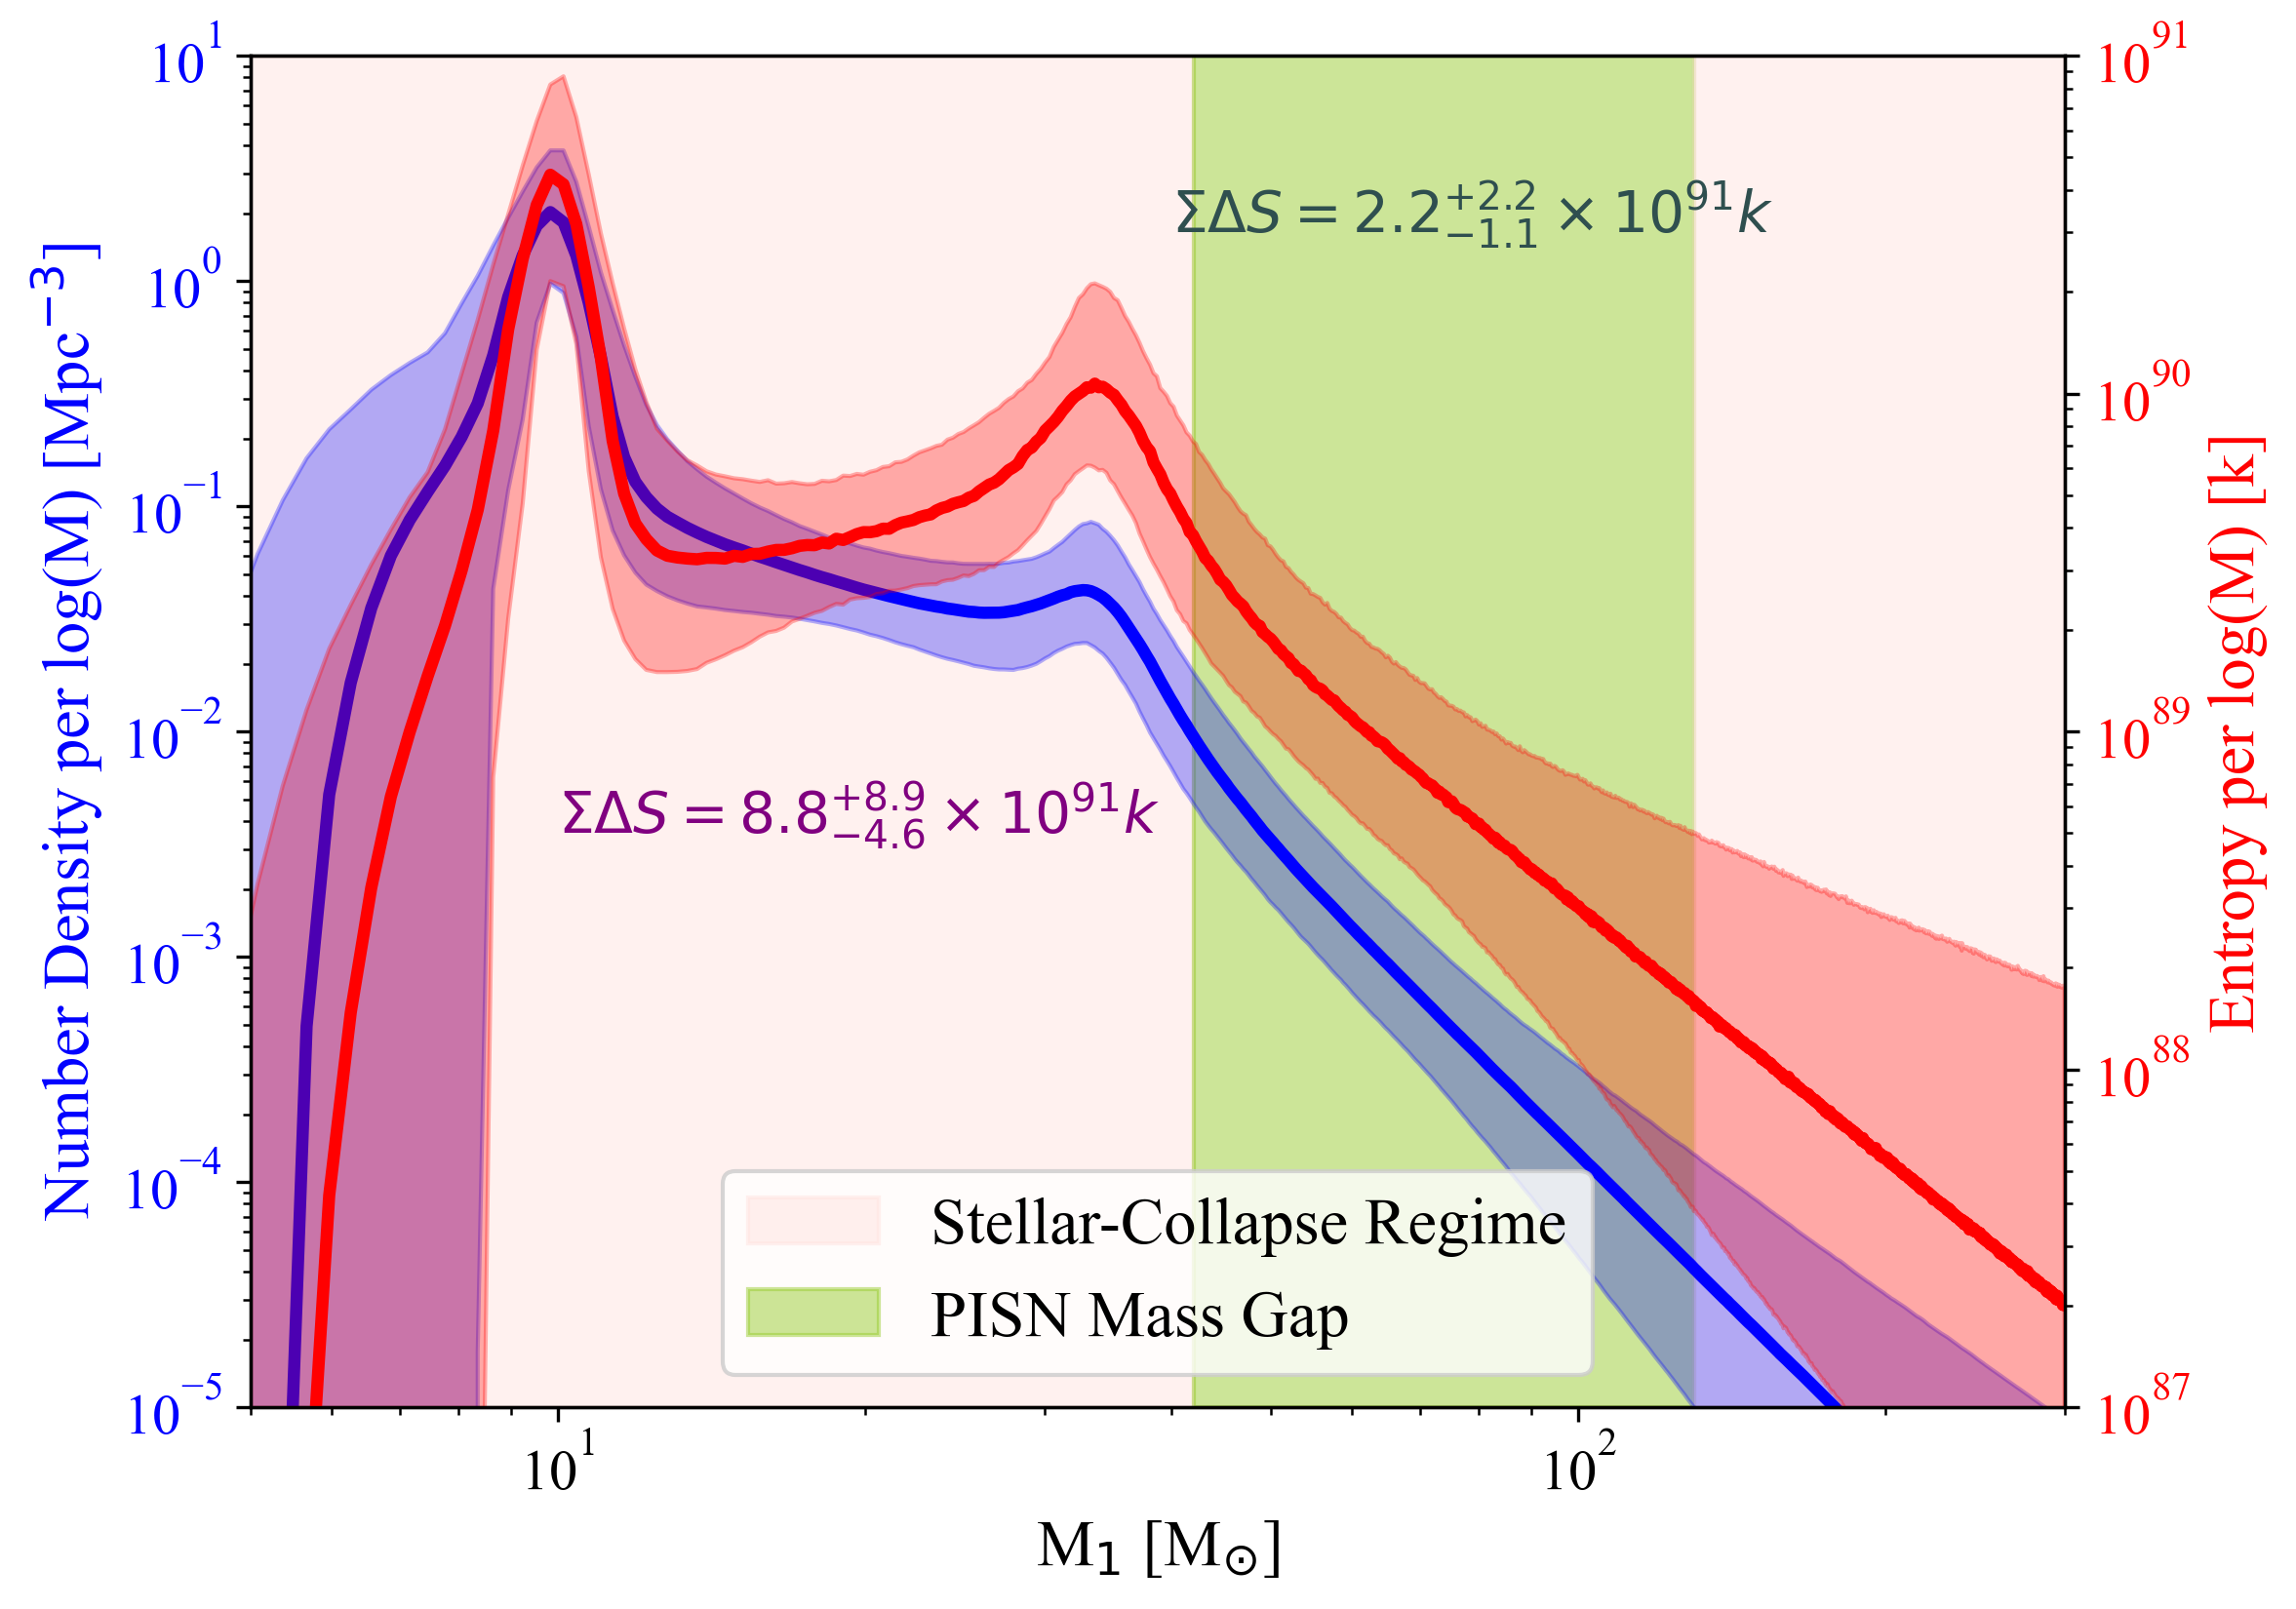
\includegraphics[width=0.48\textwidth]{num_density_entropy_gwtc4.png}
\caption{\textbf{Dynamic Entropy Production}: The blue curve (left axis) shows the GWTC-4 inferred number density of BBH mergers per Mpc$^{-3}$ per logarithmic mass interval. The red curve (right axis) shows the corresponding mass distribution of entropy generated ($\Delta S$) per $\log(M)$. We color-code the regions for PISN mass gap (yellow; $45\text{--}130~M_\odot$), while the remaining mass range (light shading) denotes the stellar-collapse regime outside the gap. Annotations report the integrated $\Sigma~\Delta S$ contributed by the two mass regimes.}
\label{fig:mass}
\end{figure}

Under this assumption, the BBH number density distribution over $5-300~M_\odot$ (blue curve in Fig. \ref{fig:mass}) closely follows the PP model calibrated to the GWTC-4 catalog. The corresponding entropy distribution (red curve in Fig. \ref{fig:mass}) inherits the characteristic double-peaked structure. In both cases the lower-mass mode dominates, but the peak-to-peak asymmetry is substantially more pronounced for the number-density distribution than for the entropy-production distribution. Specifically, at $M = 33.6~M_\odot$, the entropy increase peaks at a $\Delta S = 1.07 \times 10^{90}~k$, whereas at $M = 9.84~M_\odot$, the entropy increase peaks at $\Delta S = 4.44 \times 10^{90}~k$. As described by Eq. \ref{eq:entropy}, the entropy of a black hole scales with $S \propto M^2$. Consequently, the higher mass peak near $35~M_\odot$ is intrinsically more entropy-productive per event, but this is partially offset by its relatively lower number density compared to the peak at the lower mass near $10~M_\odot$. This interplay between mass weighting and event abundance shapes the overall entropy distribution of the observed population.

BBHs within the PISN mass gap contribute $\sim 25\%$ of the total entropy increase, even though they comprise only $1.3\%$ of the total BBH sample. This disparity highlights the outsized impact of rare, high-mass (and therefore high-entropy) events on the total merger-generated entropy budget.


In  Fig. \ref{fig:spin}, we show the population-weighted total entropy increase $\Delta S$ mapped onto the $(M_\mathrm{tot}, a_1)$ parameter space and integrated over redshift $z \in [0,20]$. The resulting structure reflects the underlying mass and spin distributions inferred from the GWTC-4 population. Because we work in total mass, we marginalize over the population distribution of the mass ratio $q$, which favors nearly equal-mass binaries ($q \simeq 1$). With this $q$-weighing, the $\Delta S$ contribution associated with the higher-mass peak ($\sim 35~M_\odot$) becomes less dominant than the primary mass representation shown in Fig. \ref{fig:mass}. While entropy production remains similarly significant across the mass range $20 - 80~M_\odot$, the double-peak structure remains obvious. 

In comparison, the spin magnitude has a weaker influence on $\Delta S$ than the masses. As indicated by Eq. \ref{eq:entropy}, the dominant scaling is $\propto M^2$, while the spin dependence is subdominant. Although the Bekenstein–Hawking entropy of an individual black hole is maximized for zero spin, the rate-weighted $\Delta S$ peaks around $a \sim 0.2$, consistent with the LVK-inferred spin distribution. This indicates that spin modulates the merger entropy budget, but the overall rate-weighted entropy production is driven primarily by the mass distribution.

\begin{figure}[t!]
\centering
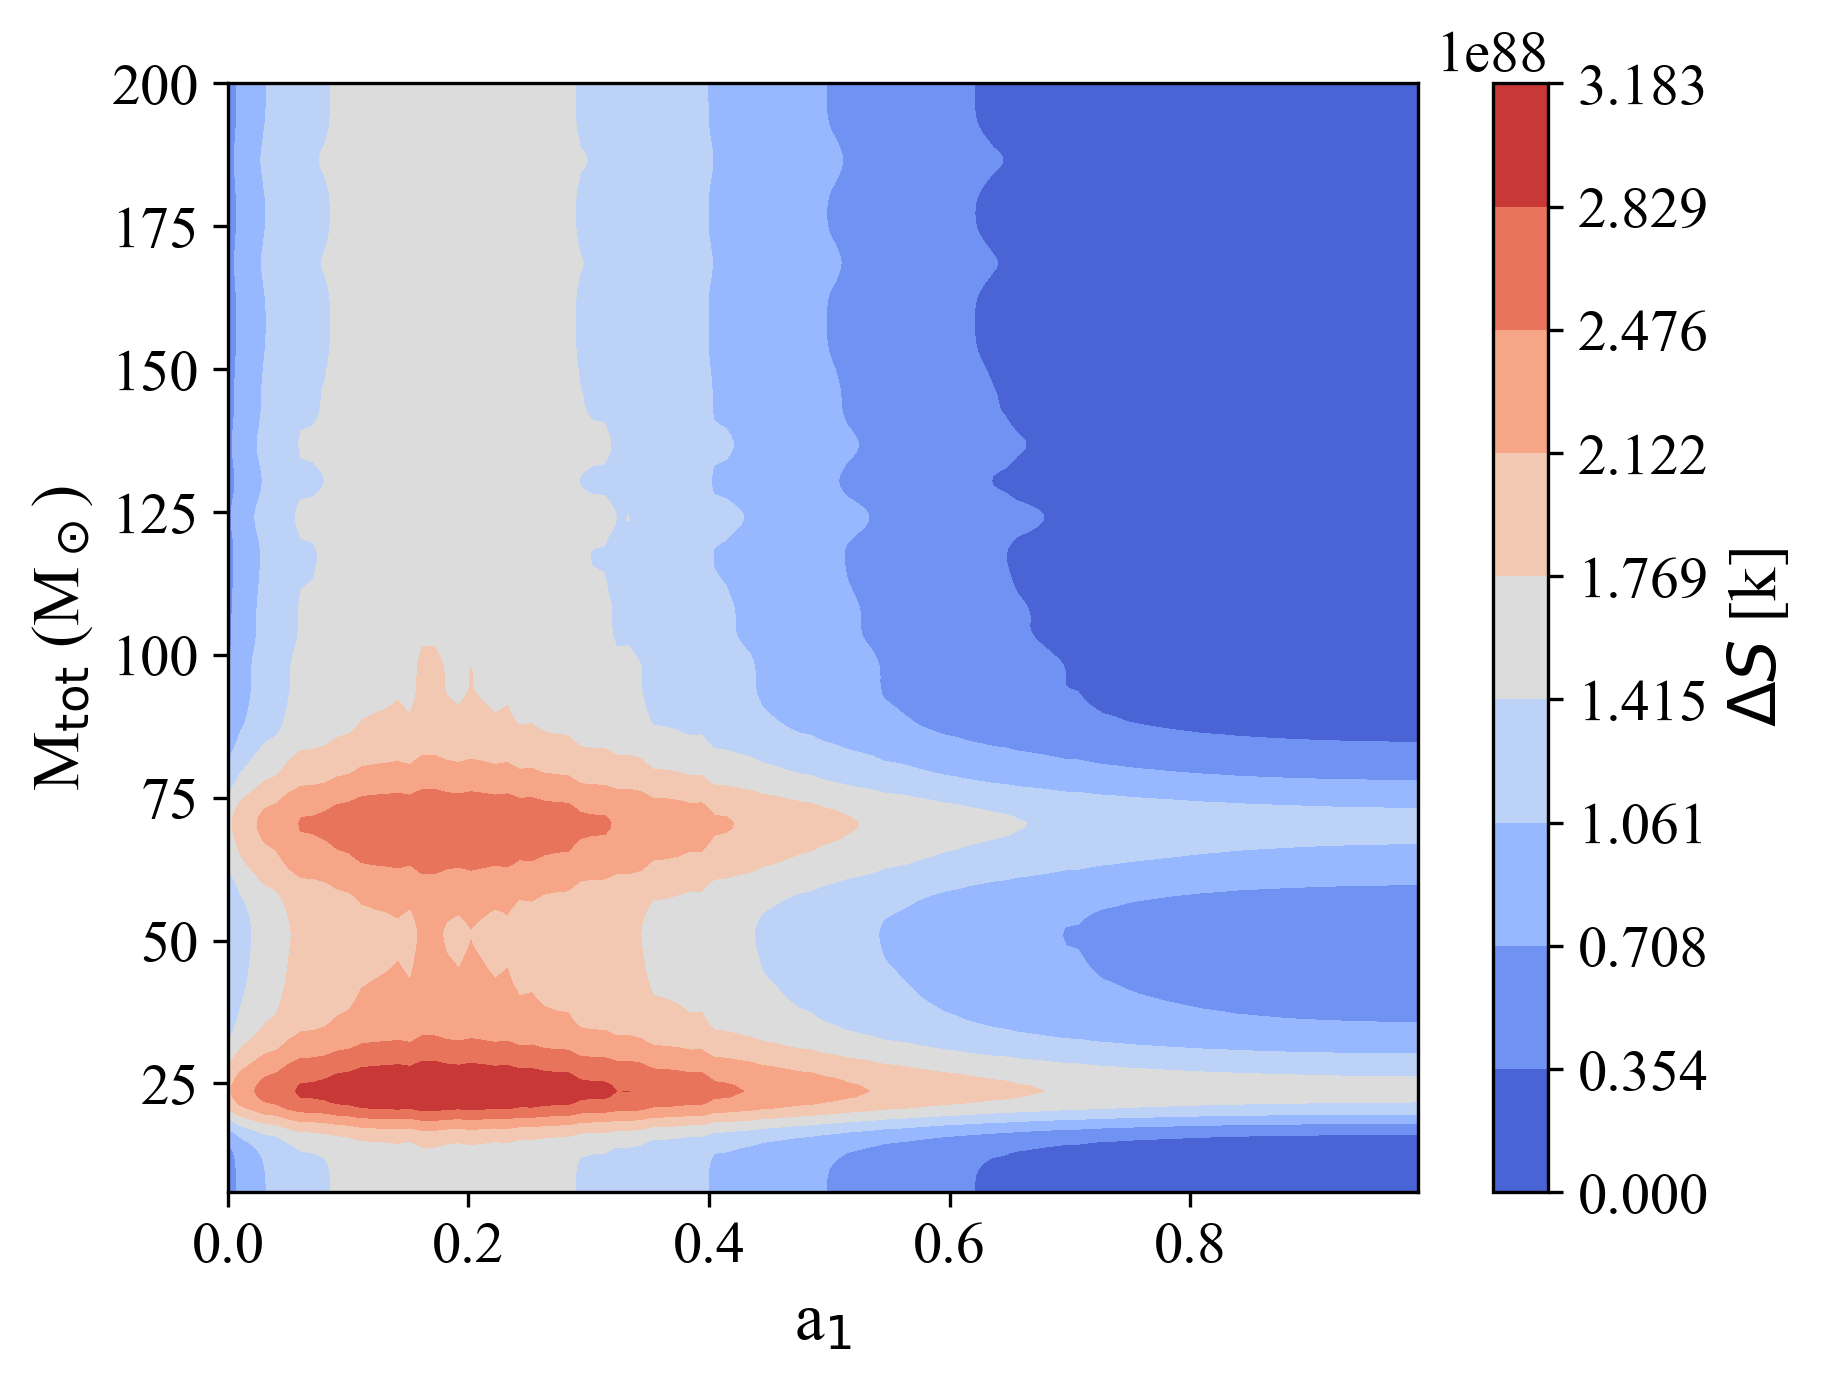
\includegraphics[width=0.5\textwidth]{spin_mass.png}
\caption{\textbf{Entropy Production in Mass-Spin Space}: the total entropy change $\Delta S$ from stellar BBH mergers across all redshift $z \in [0,20]$ in the mass ($M_\mathrm{tot}$) - spin ($a_1$) parameter space.} 
\label{fig:spin}
\end{figure}

% According to Eq. \ref{eq:entropy}, the dominant contribution scales with the square of the mass, while the spin dependence is subdominant. The entropy of a black hole is expected to be largest when the spin magnitude is 0. However, $\Delta S$ still peaks at $a \sim 0.2$, which is consistent with the spin distribution observed by LVK. This suggests that although spin contributes to the entropy budget, its role is secondary to that of mass in determining the net entropy increase from black hole mergers.


% In the PowerLaw + Peak distribution, P($m_1$ = $35~M_\odot$) $\ll$ P($m_1$ = $10~M_\odot$). However, the two peaks in $\Delta S$ are comparable in magnitude. Although there are fewer events with black holes of $35~M_\odot$ than $10~M_\odot$, the more massive BBHs lead to larger entropy magnitude, as illustrated in Eq. \ref{eq:entropy}. 
% This effect compensates for the smaller number of massive events, resulting in similar values of $\Delta S$.

% \begin{table*} [t!]
% \caption{Updated entropy budget table of different black holes with reference to previous work. The category IMBHs has lack of observational evidence to infer the total number, resulting in large error bars in the entropy estimation. \scccc{need more work on the entropy budget table}}
% \begin{ruledtabular}
% \begin{tabular}{cccc}
% Components & Entropy Density $s$ [$k~m^{-3}$] & Entropy $S~[k]$ (This Work) & Entropy $S~[k]$ (Previous Work) \\
% \hline

% Stellar BHs ($5 - 45~M_\odot$) & $2.6 \times 10^{{18}^{+0.8}_{-2.1}}$ & $9.0 \times 10^{{98}^{+0.8}_{-2.1}}$ & This Work \\

% PISN BHs ($45 - 130~M_\odot$) & $2.2^{+2.6}_{-1.5} \times 10^{12}$ & $7.9^{+9.2}_{-5.3} \times 10^{92}$ & This Work\\

% Light-IMBHs ($130 - 300~M_\odot$) & $5.1 \times 10^{18^{+0.9}_{-1.6}}$ & $1.8 \times 10^{99^{+0.9}_{-1.6}}$ & This Work \\

% IMBHs ($10^2$ - $10^{7}~M_\odot$) & $1.4 \times 10^{{17}^{+8.3}_{-1.2}}$ & $4.9 \times 10^{{97}^{+8.3}_{-1.2}}$ & \cite{frampton2009entropyintermediatemassblackholes, profumo2024newcensusuniversesentropy}\\
% % Stellar BHs (5 - 158$~M_\odot$) & $1.5^{+1.8}_{-1.1} \times 10^{16}$ & $5.4^{+5.9}_{-3.9} \times 10^{96}$ & \cite{profumo2024newcensusuniversesentropy}\\

% SMBHs ($10^{7}$ - $10^{9}~M_\odot$) & $2.4^{+3.0}_{-2.2} \times 10^{21}$ & $8.6^{+10}_{-7.8} \times 10^{101}$ & \cite{profumo2024newcensusuniversesentropy}\\


% %^{+1.8}_{-1.2}, ^{+5.9}_{-3.9}


% % Primary BH in PISN (42 - 100$~M_\odot$) & & \\
% % Secondary BH in PISN (42 - 100$~M_\odot$) & & \\
% % Remnant BH in PISN (42 - 200$~M_\odot$) & & \\
% % PISN BHs (42 - 200$~M_\odot$) & $2.2^{+2.8}_{-1.5} \times 10^{12}$ & $7.9^{+9.2}_{-5.3} \times 10^{92}$ & This Work \\
% \hline
% Entropy Produced from Merging BBHs & $1.8^{+4.5}_{-1.7} \times 10^{12}$
% & $6.3^{+15}_{-5.9} \times 10^{92}$ & This Work \\
% GWTC Pre-merger BHs (5 - 100$~M_\odot$) & $2.0^{+2.0}_{-1.2} \times 10^{12}$ & $7.0^{+6.5}_{-4.2} \times 10^{92}$ & This Work\\
% GWTC Post-merger BHs (8 - 200$~M_\odot$) & $3.1^{+3.4}_{-1.9} \times 10^{12}$ & $1.1^{+1.1}_{-6.6} \times 10^{93}$ & This Work\\

% % \textbf{PISN BHs}  & $2.8^{+8.9}_{-1.4} \times 10^{11}$
% % & $9.8^{+30}_{-9.3} \times 10^{91}$ & This Work \\
% % \hline
% % Photons & & \\
% % ISM and IGM & & \\
% % Stars & & 

% \end{tabular}
% \label{tab:budget}
% \end{ruledtabular}
% \end{table*}



Finally, we infer the redshift evolution of the merger-generated entropy using Eq. \ref{eq:growth}. The resulting total contribution per bin is shown by the blue curve in Fig. \ref{fig:growth}. We also define a localized entropy density $s(z)$ by excluding the differential comoving volume factor $\Delta V_c$, so that $s(z)$ isolates the intrinsic redshift dependence of the merger rate. $s(z)$ scales approximately with the merger rate scaled by a mass-weighted entropy-per-event factor given our uniform $t_\mathrm{lb}$ binning. Consequently, the red curve closely follows the BBH merger rate history and peaks at $z \simeq 2.79$. By contrast, the total entropy $S(z)$ retains the comoving-volume weighting through $\Delta V_c$ and therefore represents the full contribution from each redshift shell. In this sense, $S(z)$ effectively traces a volume-weighted rate, approximately $\mathcal{R}(z) \Delta V_c$. As a result, the maximum of the blue curve is shifted to higher redshift, with $S(z)$ peaking at $z\simeq 4.55$. Physically, this peak offset reflects a competition between the decline of the merger rate at high redshift and the rapid growth of the available comoving volume per redshift interval: the total contribution continues to rise beyond the intrinsic merger-rate maximum until the rate suppression outweighs the volume growth.

To quantify the redshift scaling in different regimes, we approximate the growth curve with piecewise power laws in redshift over the monotonic segments of the evolution. In the low-redshift (dark energy-influenced) regime $z \lesssim 0.5$, the total entropy growth is well described by a power law $S_\mathrm{growth} = 1.46 \times 10^{88} \times z^{2.37}$ with a tightly constrained slope from the GWTC-4 population uncertainty. At intermediate redshift ($0.5 \lesssim z \lesssim4.5$), the growth steepens ($S \propto z^{3.07}$), culminating in a maximum value of $S_\mathrm{peak} = 1.43^{+1.91}_{-0.71} \times 10^{90}~k$ at $z\simeq4.55$. Beyond the peak, the total entropy drops rapidly ($S \propto z^{-4.82}$), consistent with the sharp suppression of the merger rate at higher redshift.


\begin{figure}[t!]
\centering
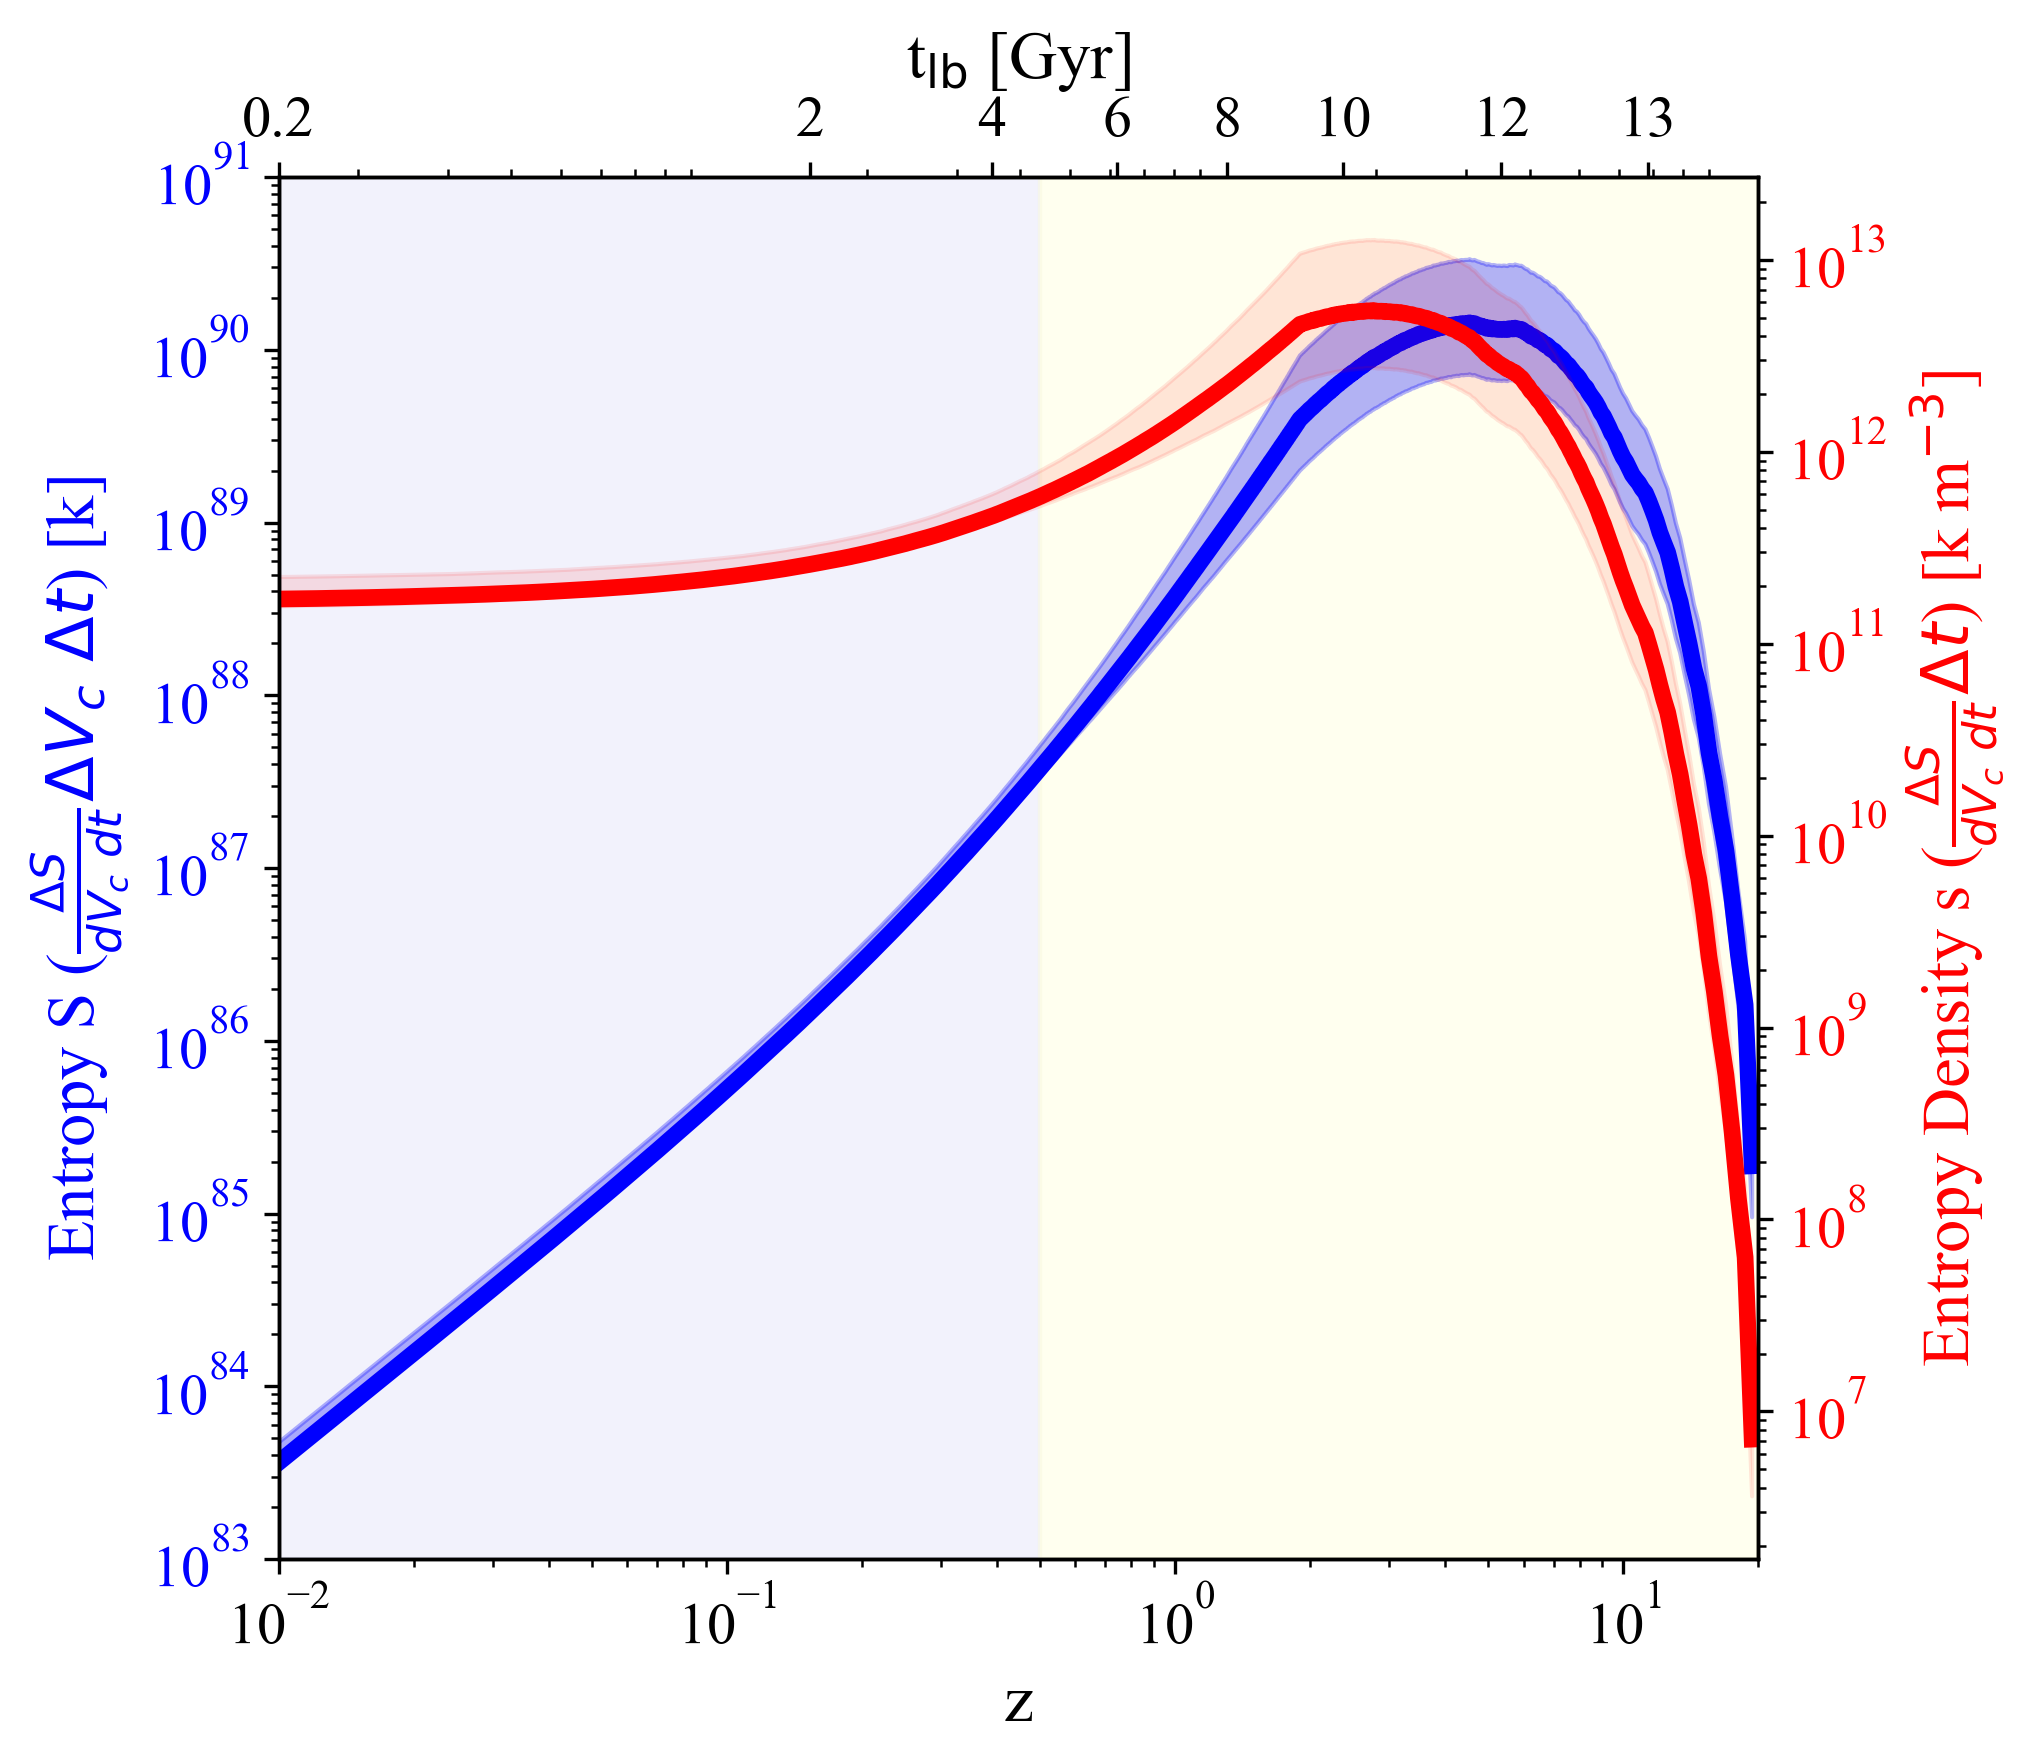
\includegraphics[width=0.48\textwidth]{growth_entropy_gwtc4_only.png}
\caption{\textbf{Cosmic History of Merger-Generated Entropy}: total entropy (left y axis \& blue curve) and entropy density (right y axis \& red curve) from merging BBHs in the comoving frame across $z \in [0.01, 20]$, as a function of the redshift $z$ (bottom x axis) and of the look-back time $t_{lb}$ (top x axis). 
% The blue curve represents the total entropy %($\frac{\Delta S}{dV_c~dt}\Delta V_c~\Delta t$) 
% with error bars, where we use the BBH merger rate to multiply the differential comoving volume $dV$ and differential lookback time $dt$ to infer the growth entropy. The red curve represents the growth entropy density 
% %($\frac{\Delta S}{dV_c~dt}\Delta t$) 
% with error bars, where only $dt$ is taken into account. 
The dark energy-dominated and matter-dominated eras are shaded purple and yellow, respectively.}
\label{fig:growth}
\end{figure}
% Finally, we infer the redshift evolution of entropy growth from BBH mergers using Eq. \ref{eq:growth}, shown as the blue curve in Fig. \ref{fig:growth}. The localized entropy density (plotted in red), which excludes the differential comoving volume factor $\Delta V_c$, traces the redshift distribution of the BBH merger rate. This consistency arises because the redshift bins are uniform in lookback time, effectively aligning the entropy density with the distribution of merger rate. The red curve is scaled by the entropy increased per merger event. In contrast, the total entropy includes the $\Delta V_c$ factor and accounts for the expanding comoving volume at higher redshifts. As a result, the peak of the total entropy distribution shifts from $z \sim 2.79$ to $z \sim 4.55$.

% From Fig. \ref{fig:growth}, we observe that the entropy in the dark energy-dominated region follows a power law behavior. By performing a numerical fit, we find that the correlation between the growth entropy $S_\mathrm{growth}$ and redshift 
% $z$ is well described by:

% \begin{equation}
% \centering
%     S_\mathrm{growth} = 1.635 \times 10^{88} \times z^{2.496}
% \end{equation}

% In the matter-dominated era, the entropy increases more rapidly, reaching a maximum of $2.91^{+7.23}_{-2.74} \times 10^{90}~k$ at $z \sim 4.55$, before dropping sharply due to lower merger rates at higher redshifts. Although the merger rate itself peaks around $z \sim 2.79$, the continued rise in entropy growth beyond this redshift is driven by the increase in differential comoving volume at earlier cosmic times. This volume factor effectively shifts the peak of the entropy distribution to higher redshifts, decoupling it from the peak of the merger rate alone.

Building on our new calculations, we revisit the entropy census of major cosmic components using the budget compiled by \cite{Egan_2010} as a reference baseline. Over the past decade, surveys and missions have substantially refined several inputs to this census, including the observational confirmation by the LVK Collaboration of heavier stellar black holes in the $\sim 45-130~M_\odot$ range. Incorporating these updates, together with additional components considered in more recent work, we present a revised and expanded entropy budget of the observable universe in Table \ref{tab:budget}. This compilation extends earlier inventories \citep{Frautschi1982, Frampton_2008, frampton2009entropyintermediatemassblackholes, Frampton_2009, Egan_2010, profumo2024newcensusuniversesentropy} by adopting updated estimates where available and providing references for each entry. In particular, we explicitly include the contribution associated with BBH mergers, which emerges as a substantial component of the late-time thermodynamic budget.

\begin{figure*}[t!]
\centering
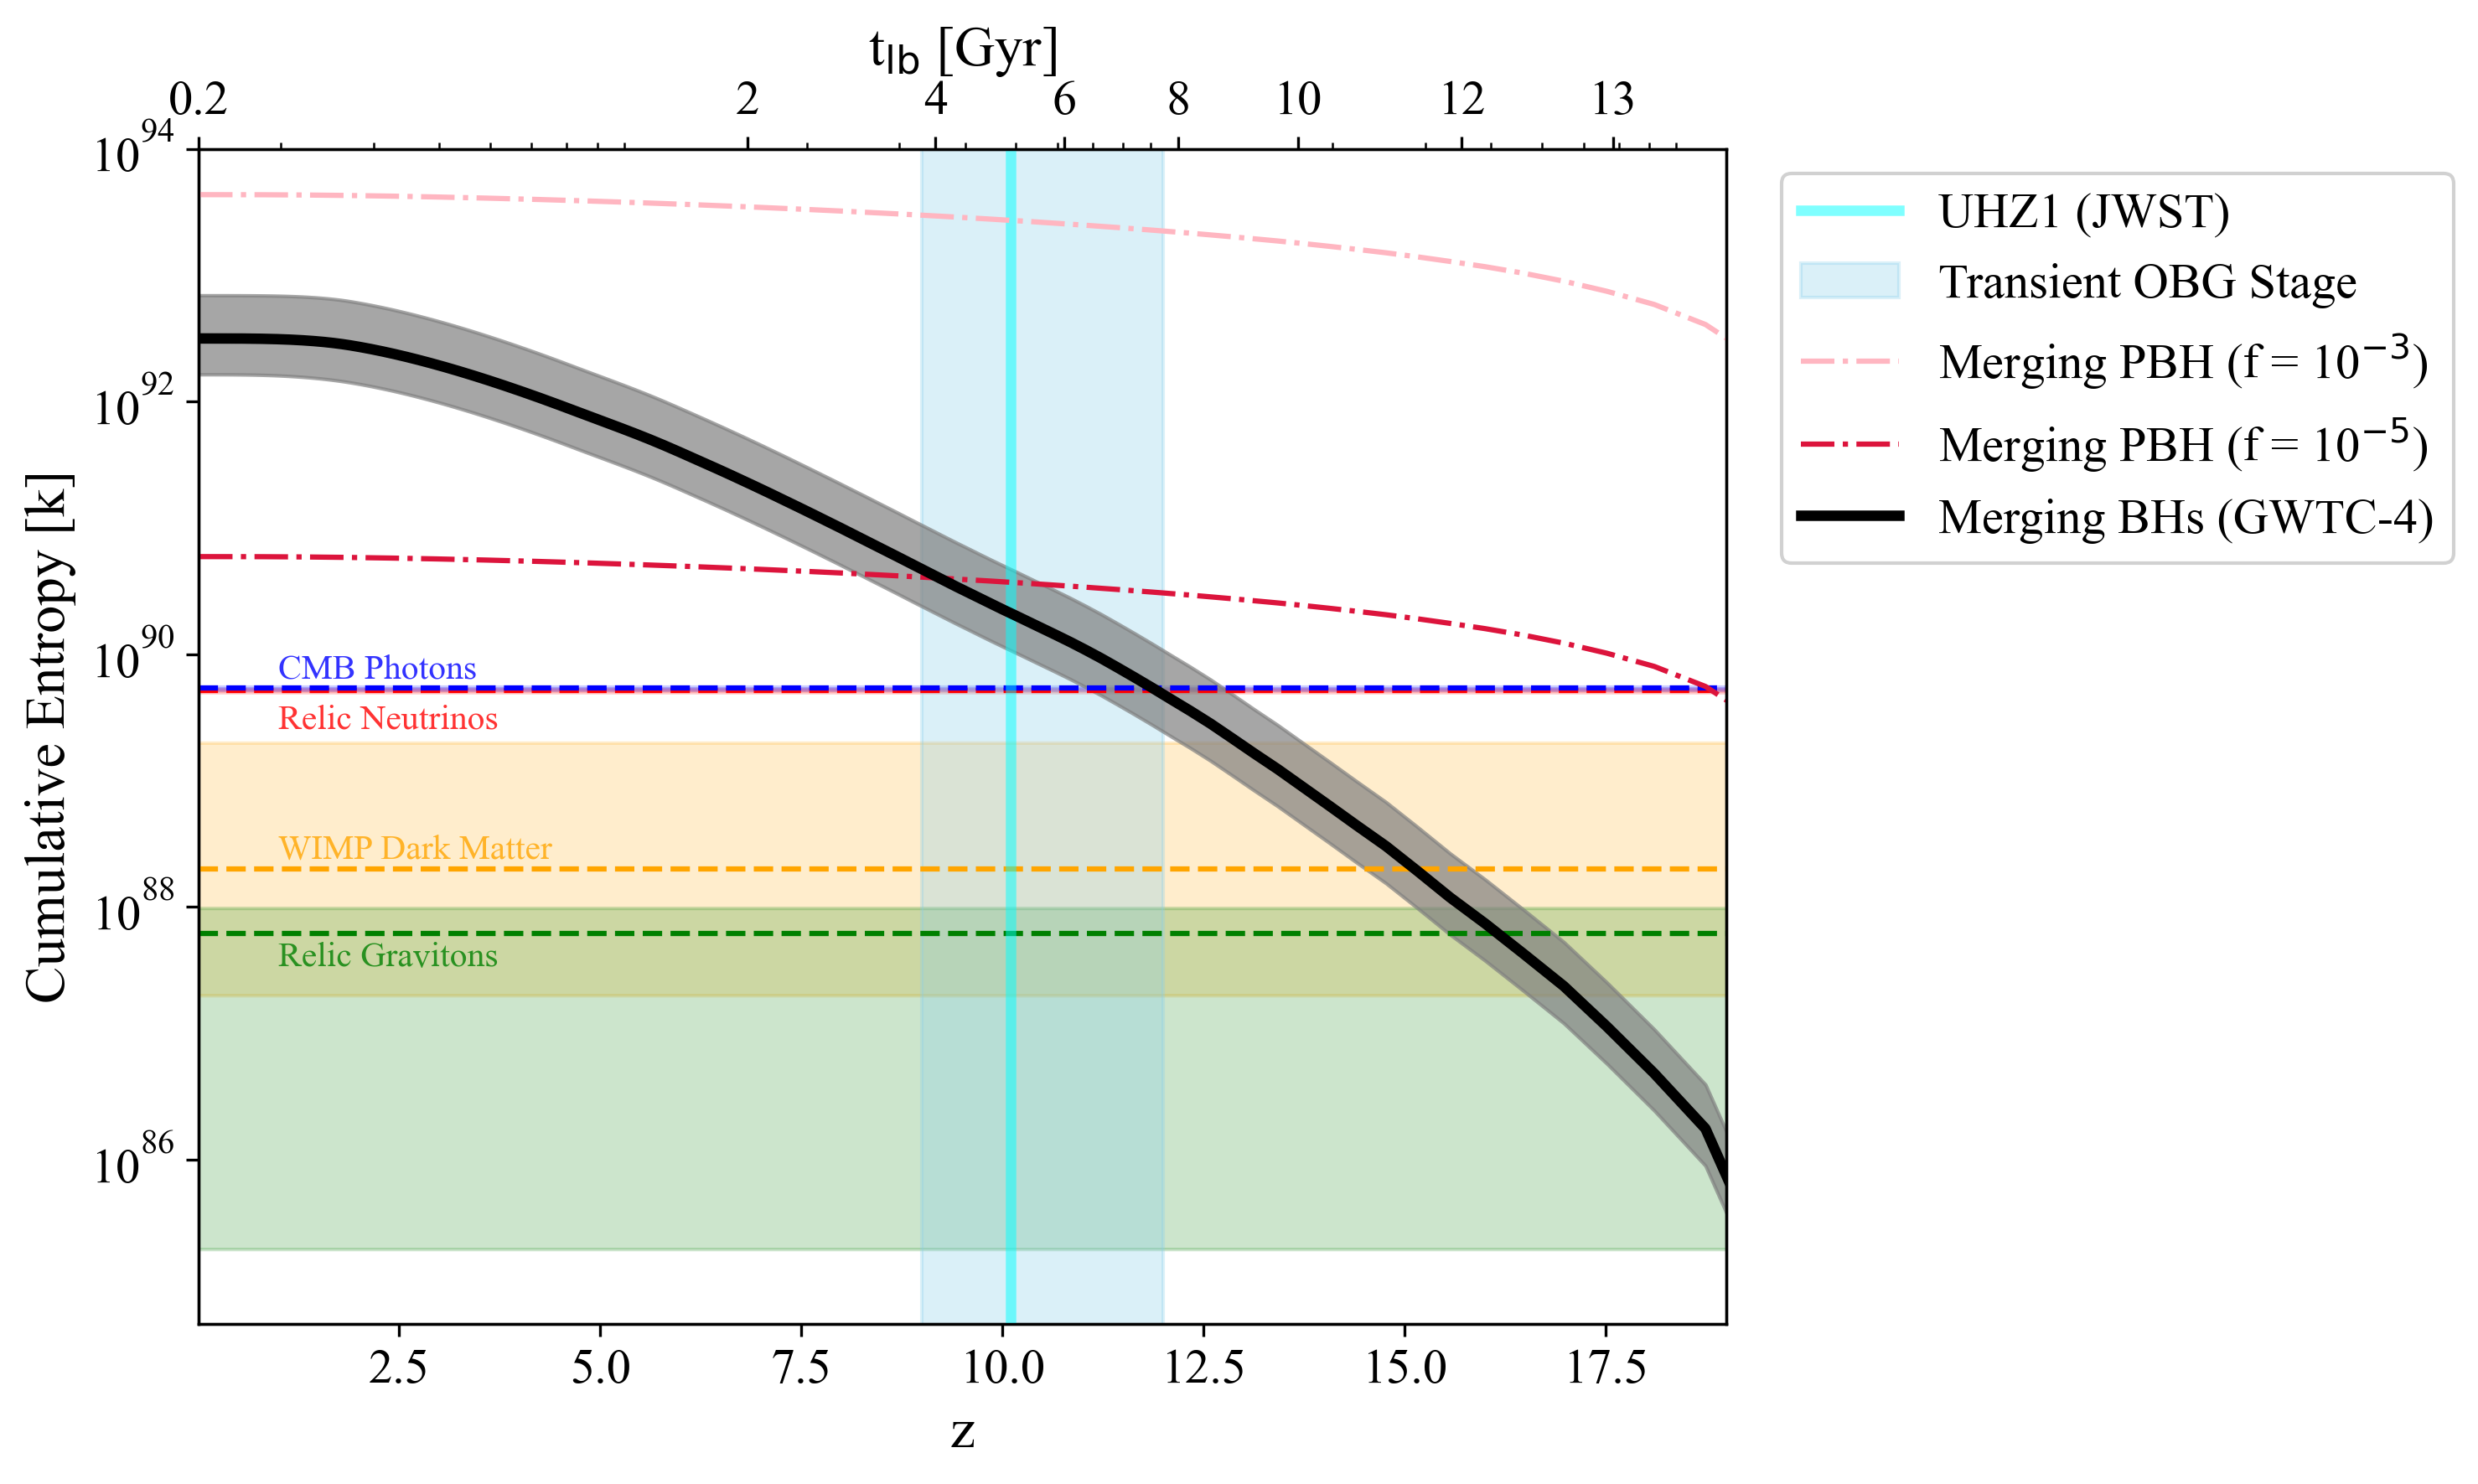
\includegraphics[width=0.9\textwidth]{cumulative_tot_ent_gwtc4_pbh.png}
\caption{\textbf{Cumulative Cosmological Entropy Budget}: cumulative entropy from merging BBHs in the comoving frame as a function of redshift over $z \in [0.01,20]$. For comparison, we also show the entropy contribution from PBHs for two PBH fraction choices. For reference, the entropy contributions from other cosmic components, as estimated in \cite{Egan_2010}, are included. The vertical line marks the redshift of the most distant black hole observed by JWST in galaxy UHZ1, and the shaded vertical band indicates the transient OBG stage associated with this epoch. \label{fig:pbh?}}
\end{figure*}

% The cosmological density parameter associated to GW loss is $\Omega_\mathrm{GW} = 5.01^{+6.50}_{-2.85} \times 10^{-11}$. In comparison to the baryon densities like cosmic microwave background (CMB) photons $\Omega_\gamma \approx 5 \times 10^{-5}$ and neutrinos $\Omega_\nu \approx 3.4 \times 10^{-5}$, our estimate is six orders of magnitude smaller. While black holes have overtaken the universe in terms of entropy, energy of photons is much larger than that released from merging BBHs. Most mass-energy still retained in the remnant black holes because the merger process is extremely efficient at conserving mass-energy within the event horizon. In accordance with the First Law of Thermodynamics, the progenitor mass is conserved, partitioned between the remnant black hole ($\Omega_\mathrm{BH,rem} \sim 10^{-9}$) and the radiated energy ($\Omega_{GW} \sim 10^{-11}$). In accordance with the Second Law, this small release of energy facilitates a disproportionately large increase in entropy. Thus, we interpret $\Omega_{GW}$ not merely as a background radiation field, but as the necessary energetic by-product of the universe's drive toward its maximum entropy state.



\section{Cosmological Implications}
\label{sec:cumulation+rate}


% \subsection{Entropy from GWTC-3 Merging Black Holes}
% \scccc{Compare two regions}
% \subsection{Entropy Density Rate}
% In Fig. \ref{fig:growth}, we show the growth entropy and growth entropy density, which is computed with Eqs. \ref{eq:growth} and \ref{eq:density}. The growth entropy density is consistent with the distribution of BBH merger rate. The growth entropy incorporates a factor of $\Delta V_c$. Similarly, the growth entropy density reaches the maximum at $z \sim 2.79$. 


% In the matter-dominated region, the growth entropy increases more rapidly until $z \sim 4.55$, when growth entropy reaches $2.91^{+7.23}_{-2.74} \times 10^{90}~k$. Then the growth entropy rapidly drops due to lower merger rate. Although the merger rate peaks $z \sim 2.79$, entropy growth continues to increase due to larger differential volume. The volume factor shifts the growth entropy peak further to higher redshifts. 

% The growth entropy reaches the maximum at $z=4.55$. The differential comoving volume $\Delta V_c$

% \begin{figure}[t!]
% \centering
% \includegraphics[width=0.49\textwidth]{cumulative_tot_ent.png}
% % \includegraphics[width=0.49\textwidth]{cumulative_ent_den.png}
% \caption{Cumulative entropy from merging BBHs in the comoving frame over the redshift range $z \in [0.01,20]$, shown as a function of the redshift $z$ (bottom x axis) and of the look-back time $t_{lb}$ (top x axis).  For reference, the total entropy contributions from other cosmic components, as estimated in \cite{Egan_2010}, are also shown. The vertical line marks the redshift of the most distant galaxy observed by JWST. The purple-shaded region corresponds to the dark energy–dominated era ($z \le 0.5$), while the yellow-shaded region represents the matter-dominated era ($z > 0.5$).}
% \label{fig:cumulative}
% \end{figure}

% \begin{figure*}[t!]
% \centering
% \includegraphics[width=0.49\textwidth]{cumulative_tot_ent_gwtc4.png}
% \includegraphics[width=0.49\textwidth]{cumulative_ent_den_gwtc4.png}
% \caption{The left panel shows the cumulative entropy, and the right panel shows the entropy density rate (as defined in Sec. \ref{sec:cumulation+rate}) from merging BBHs in the comoving frame over the redshift range $z \in [0.01,20]$. Both quantities are plotted as functions of redshift  $z$ (bottom x axis) and look-back time $t_{lb}$ (top x axis). For reference, the entropy contributions from other cosmic components, as estimated in \cite{Egan_2010}, are also included. The purple-shaded region corresponds to the dark energy–dominated era ($z \le 0.5$), while the yellow-shaded region represents the matter-dominated era ($z > 0.5$). In the left panel, the vertical line marks the redshift of the most distant black hole observed by JWST in galaxy UHZ1, and the shaded vertical band indicates the transient OBG stage associated with this epoch.
% %The blue curve represents the total growth entropy ($\frac{\Delta S}{\Delta V \Delta t} dt dV$), where we use the BBH merger rate to multiply the differential comoving volume $dV$ and differential lookback time $dt$. The red curve represents the growth entropy density ($\frac{\Delta S}{\Delta V \Delta t}dt$). The scale of total growth entropy and entropy density are shown in the two vertical axes.
% \label{fig:rate}
% }
% \end{figure*}



To evaluate the cumulative entropy contribution from BBH mergers since the Big Bang, we integrate the differential entropy growth (blue curve in Fig. \ref{fig:growth}) from the highest redshifts down to the present epoch. The resulting cumulative entropy $\mathcal{S}_{\rm BH}(z)$ is shown in Fig. \ref{fig:pbh?}. This metric captures the cumulative, irreversible entropy from BBH mergers across cosmic time, quantifying their contribution to the cosmic entropy budget from the earliest structure formation epochs to today.

\subsection{The Thermodynamic Crossover at Cosmic Dawn}
\label{subsec:cmb_cross}
As shown in Fig. \ref{fig:pbh?}, the cumulative entropy increases monotonically, as expected for an integrated entropy-generation history. A salient feature of this evolution is the ``thermodynamic crossover,'' where the cumulative entropy produced by mergers exceeds the total entropy of the CMB photons. We find that this transition occurs at a redshift of $z = 12.6^{+1.5}_{-3.5}$. This result indicates that the cumulative merger-associated entropy becomes comparable to, and then exceeds, the CMB photon entropy budget significantly earlier than the peak of cosmic star formation, suggesting that merger-driven entropy accumulation is already substantial during Cosmic Dawn in this reference comparison.
% essentially establishing thermodynamic dominance during the epoch of Cosmic Dawn.

This crossover is particularly intriguing in the context of high-redshift observations. The James Webb Space Telescope (JWST) has reported the detection of an accreting black hole with mass $M_\mathrm{BH} \sim 4 \times 10^7~M_\odot$ in the galaxy UHZ1 at $z \sim 10.1$ \citep{natarajan2023detectionovermassiveblackhole}. Theoretical models predict a transient phase of over-massive black hole galaxies (OBGs) over $z \in [9,12]$ \citep{2013MNRAS.432.3438A, Natarajan_2017}, which is highlighted in the figure (blue shaded region). Intriguingly, the cumulative entropy from BBH mergers is found to exceed that of the CMB around the onset of this transient OBG stage. While this temporal proximity does not imply a causal connection, it is consistent with scenarios in which BBH mergers contribute a non-negligible share of the cumulative entropy generated by $z \gtrsim 10$. In particular, it may be compatible with light-seed models in which Population III remnants produce black hole seeds in the mass range $10$-$100~M_\odot$. These seeds form at very high redshift, participate in hierarchical mergers, and may contribute to the assembly of the massive black holes inferred in JWST observations. The strength of this inference, however, depends on the assumed high-redshift BBH merger rate and on the entropy-generation prescription adopted for mergers.
% This suggests that black hole mergers were already contributing significantly to the thermodynamic state of the universe during this early epoch, potentially supporting light seed models in which Population III stars collapse into black hole seeds in the mass range of $10-100~M_\odot$. These seeds, formed in the infant universe, dominate the entropy budget at $z \gtrsim 12$, actively participate in hierarchical mergers, and serve as the building blocks for SMBHs observed by JWST.

\subsection{Constraints from the Dark Ages: The PBH Floor}
Our analysis primarily focuses on the stellar-origin BBH population, which is expected to be negligible at very high redshift, prior to the onset of Population III star formation (and our results are shown over the range highlighted in the data $z\le20$). In the absence of additional channels, the merger-generated entropy in this regime therefore approaches a minimal baseline set by the stellar contribution alone. If PBHs constitute a non-zero fraction of the dark matter, PBH binaries can form and merge well before the first stars ignite, thereby establishing an ``entropy floor” for the cumulative merger-generated gravitational entropy at high redshift.


The magnitude of this floor depends sensitively on the PBH abundance, $f_\mathrm{PBH} \equiv \Omega_\mathrm{PBH}/\Omega_\mathrm{DM}$, and on the PBH mass function. Low-mass PBHs ($M \ll 1~M_\odot$) contribute negligibly to the merger-generated entropy budget considered here even for $f_\mathrm{PBH} \sim 1$ because the characteristic black-hole entropy scales steeply with mass. By contrast, stellar-mass PBHs in the LVK-relevant range ($M \sim 30~M_\odot$) carry a much larger entropy per merger event and can substantially enhance the cumulative entropy from mergers. In this study, we consider two representative abundances: a higher-abundance case ($f_\mathrm{PBH} = 10^{-3}$, pink dot-dashed line) and a conservative low-abundance case ($f_\mathrm{PBH} = 10^{-5}$, red dot-dashed line). The resulting cumulative entropy histories are shown in Fig.~\ref{fig:pbh?} and compared directly to the stellar-origin BBH contribution.

As illustrated by the $f_\mathrm{PBH} = 10^{-3}$ case, the PBH merger contribution exceeds the stellar-origin BBH contribution across the full $z$ range shown, implying that the merger-generated entropy budget is PBH-dominated in this scenario. This behavior is a direct consequence of the efficient early-time mergers of primordial binaries, with a rate scaling $\mathcal{R}(t) \propto t^{-34/37}$ \citep{Sasaki_2016}, which enables substantial entropy accumulation already at very high redshift. Consequently, the stellar channel remains sub-dominant in cumulative merger-generated entropy at all epochs displayed.

The lower-abundance case ($f_\mathrm{PBH} = 10^{-5}$) yields a more dynamic thermodynamic history. Even at this level, PBH mergers can accumulate entropy early, surpassing the entropy budget of CMB photons as early as $z \sim 18.7$. As cosmic structure formation proceeds, the stellar-origin BBH merger rate rises rapidly, and the cumulative stellar contribution eventually intersects and overtakes the PBH contribution. We find a crossover at $z=9.17^{+1.31}_{-1.01}$, after which the cumulative merger-generated entropy is driven primarily by astrophysical black holes. This delineates two regimes in the merger-generated entropy history for $f_\mathrm{PBH} \sim 10^{-5}$: a PBH-dominated phase at earlier times followed by a stellar-dominated phase toward lower redshift.

\subsection{Cosmological Density Parameters \& Thermodynamic Asymmetry}
Beyond the entropy census, we compute the cosmological density parameters of the black hole population to quantify the energetic footprint.

We first estimate the mass-energy inventory stored in stellar-origin black holes. We find an initial mass density parameter of $\Omega_\mathrm{BH} = 5.32^{+6.65}_{-3.37}\times 10^{-5}$, which is consistent with typical local-universe estimates ($\sim 10^{-5}$). The modest offset is expected given our assumption of a uniformly low-metallicity population ($Z=2\times 10^{-4}$): weaker line-driven winds reduce stellar mass loss, leading to systematically heavier compact remnants and a larger inferred black hole mass density.

Only a small fraction of this population undergoes mergers. We infer the mass density in merger remnants to be $\Omega_\mathrm{BH,~rem} = 4.19^{+5.68}_{-2.44} \times 10^{-9}$. The ratio $\Omega_\mathrm{BH,~rem}~/~\Omega_\mathrm{BH} \sim 8 \times 10^{-5}$ indicates that only a tiny fraction of the stellar black-hole mass budget has been processed through BBH mergers to date. Integrating the merger history, we find a GW energy density parameter of $\Omega_\mathrm{GW} = 5.01^{+6.50}_{-2.85}\times 10^{-11}$, approximately six orders of magnitude below the energy densities of standard relativistic components, such as CMB photons ($\Omega_{\gamma} \approx 5 \times 10^{-5}$) or neutrinos ($\Omega_{\nu} \approx 3.4 \times 10^{-5}$).

Thus, although black holes dominate the late-time entropy budget, the Universe’s energy budget remains overwhelmingly carried by radiation rather than by merger-generated GWs. The origin of this disparity is that BBH mergers radiate only a small fraction of the system’s mass-energy, with most of the energy remaining behind the horizon in the remnant black hole. We find $\Omega_\mathrm{GW}/\Omega_\mathrm{BH,rem} \sim 10^{-2}$, consistent with the modest radiative efficiency of BBH mergers. Yet even this small radiated fraction can accompany a large entropy increase in accord with the second law. These results illustrate a \textit{thermodynamic asymmetry} in black hole mergers:
\begin{enumerate}
    \item \textbf{Energetically Inefficient:} BBH mergers radiate only a minute fraction of their mass-energy ($\Omega_\mathrm{GW}/\Omega_\mathrm{BH,rem} \sim 10^{-2}$) and contribute negligibly to the universe's energy budget compared to radiation or matter.
    \item \textbf{Entropically Dominant:} Conversely, as demonstrated in Sec. \ref{subsec:cmb_cross}, these same events drive a disproportionate increase in cosmic entropy, surpassing the CMB photon entropy budget at $z \sim 12$.
\end{enumerate}
Therefore, we interpret $\Omega_\mathrm{GW}$ not as a major energy component, but as the unavoidable energetic by-product of an irreversible process that efficiently advances the universe toward a higher-entropy state.


\subsection{Volume-normalized Retrospective Entropy Density}

To characterize the volumetric accumulation of entropy, we compute the cumulative number of BBH mergers enclosed within $z$ by integrating the merger-rate density over the past light cone:

\begin{equation}
    \centering
    N_\mathrm{BBH}(z) = \int_{0}^{z} \mathcal{R}(z)~dV_c(z)~dt_\mathrm{lb}(z)
    \label{eq:cumulative}
\end{equation}

We then introduce a new quantity termed \textit{retrospective entropy density}, a volume-normalized cumulative measure that compares the total merger-generated entropy integrated over $z \in [0.01, z_0]$ to the comoving volume enclosed within the same interval:

\begin{equation}
    \mathrm{Retrospective~Entropy~Density~(z_0)} = \frac{\sum^{\mathrm{N_{BBH}(z_0)}}_{i=1} \Delta S_i}{\int^{z_0}_0 dV_{c}(z)}
    \label{eq:rate_entropy_density}
\end{equation}

Geometrically, this definition corresponds to constructing concentric comoving spheres centered on the observer (the present epoch), each extending out to a maximum redshift $z_0$. The numerator represents the cumulative entropy produced by all BBH mergers occurring within that past-light-cone volume, while the denominator provides the corresponding comoving volume normalization. We emphasize that this quantity is \emph{not} the instantaneous physical entropy density at redshift $z_0$. Rather, it serves as a retrospective accounting metric, quantifying the average density of merger-driven entropy associated with the spacetime region enclosed by $z_0$. The resulting evolution is shown in Fig. \ref{fig:rate}.

Since both the cumulative entropy $\Sigma~\Delta S$ and the enclosed comoving volume $V_c(<z)$ increase monotonically with redshfits, their ratio elucidates the competition between entropy accumulation and the expansion of the accessible volume. In our reconstruction based on GWTC-4, the retrospective entropy density rises from the local Universe to reach a maximum of $4.17^{+5.35}_{-2.00} \times 10^{12}~k~m^{-3}$ at $z = 4.33^{+0.08}_{-0.12}$, before declining toward higher redshifts. This peak reflects the interplay between (i) the growing cumulative contribution from mergers as the integration extends to earlier cosmic times, and (ii) the rapid geometric growth of the enclosed comoving volume, which dilutes the volume-normalized ratio once the merger contribution ceases to grow at a comparable rate. As $z$ approaches the upper bound ($z \simeq 20$), the retrospective entropy density asymptotes to the average comoving entropy density contributed by BBH mergers in the observable universe, consistent with the value reported in Table \ref{tab:budget}.


\label{subsec:retro_den}
\begin{figure}[t!]
% \centering
% \includegraphics[width=0.49\textwidth]{cumulative_tot_ent_gwtc4.png}
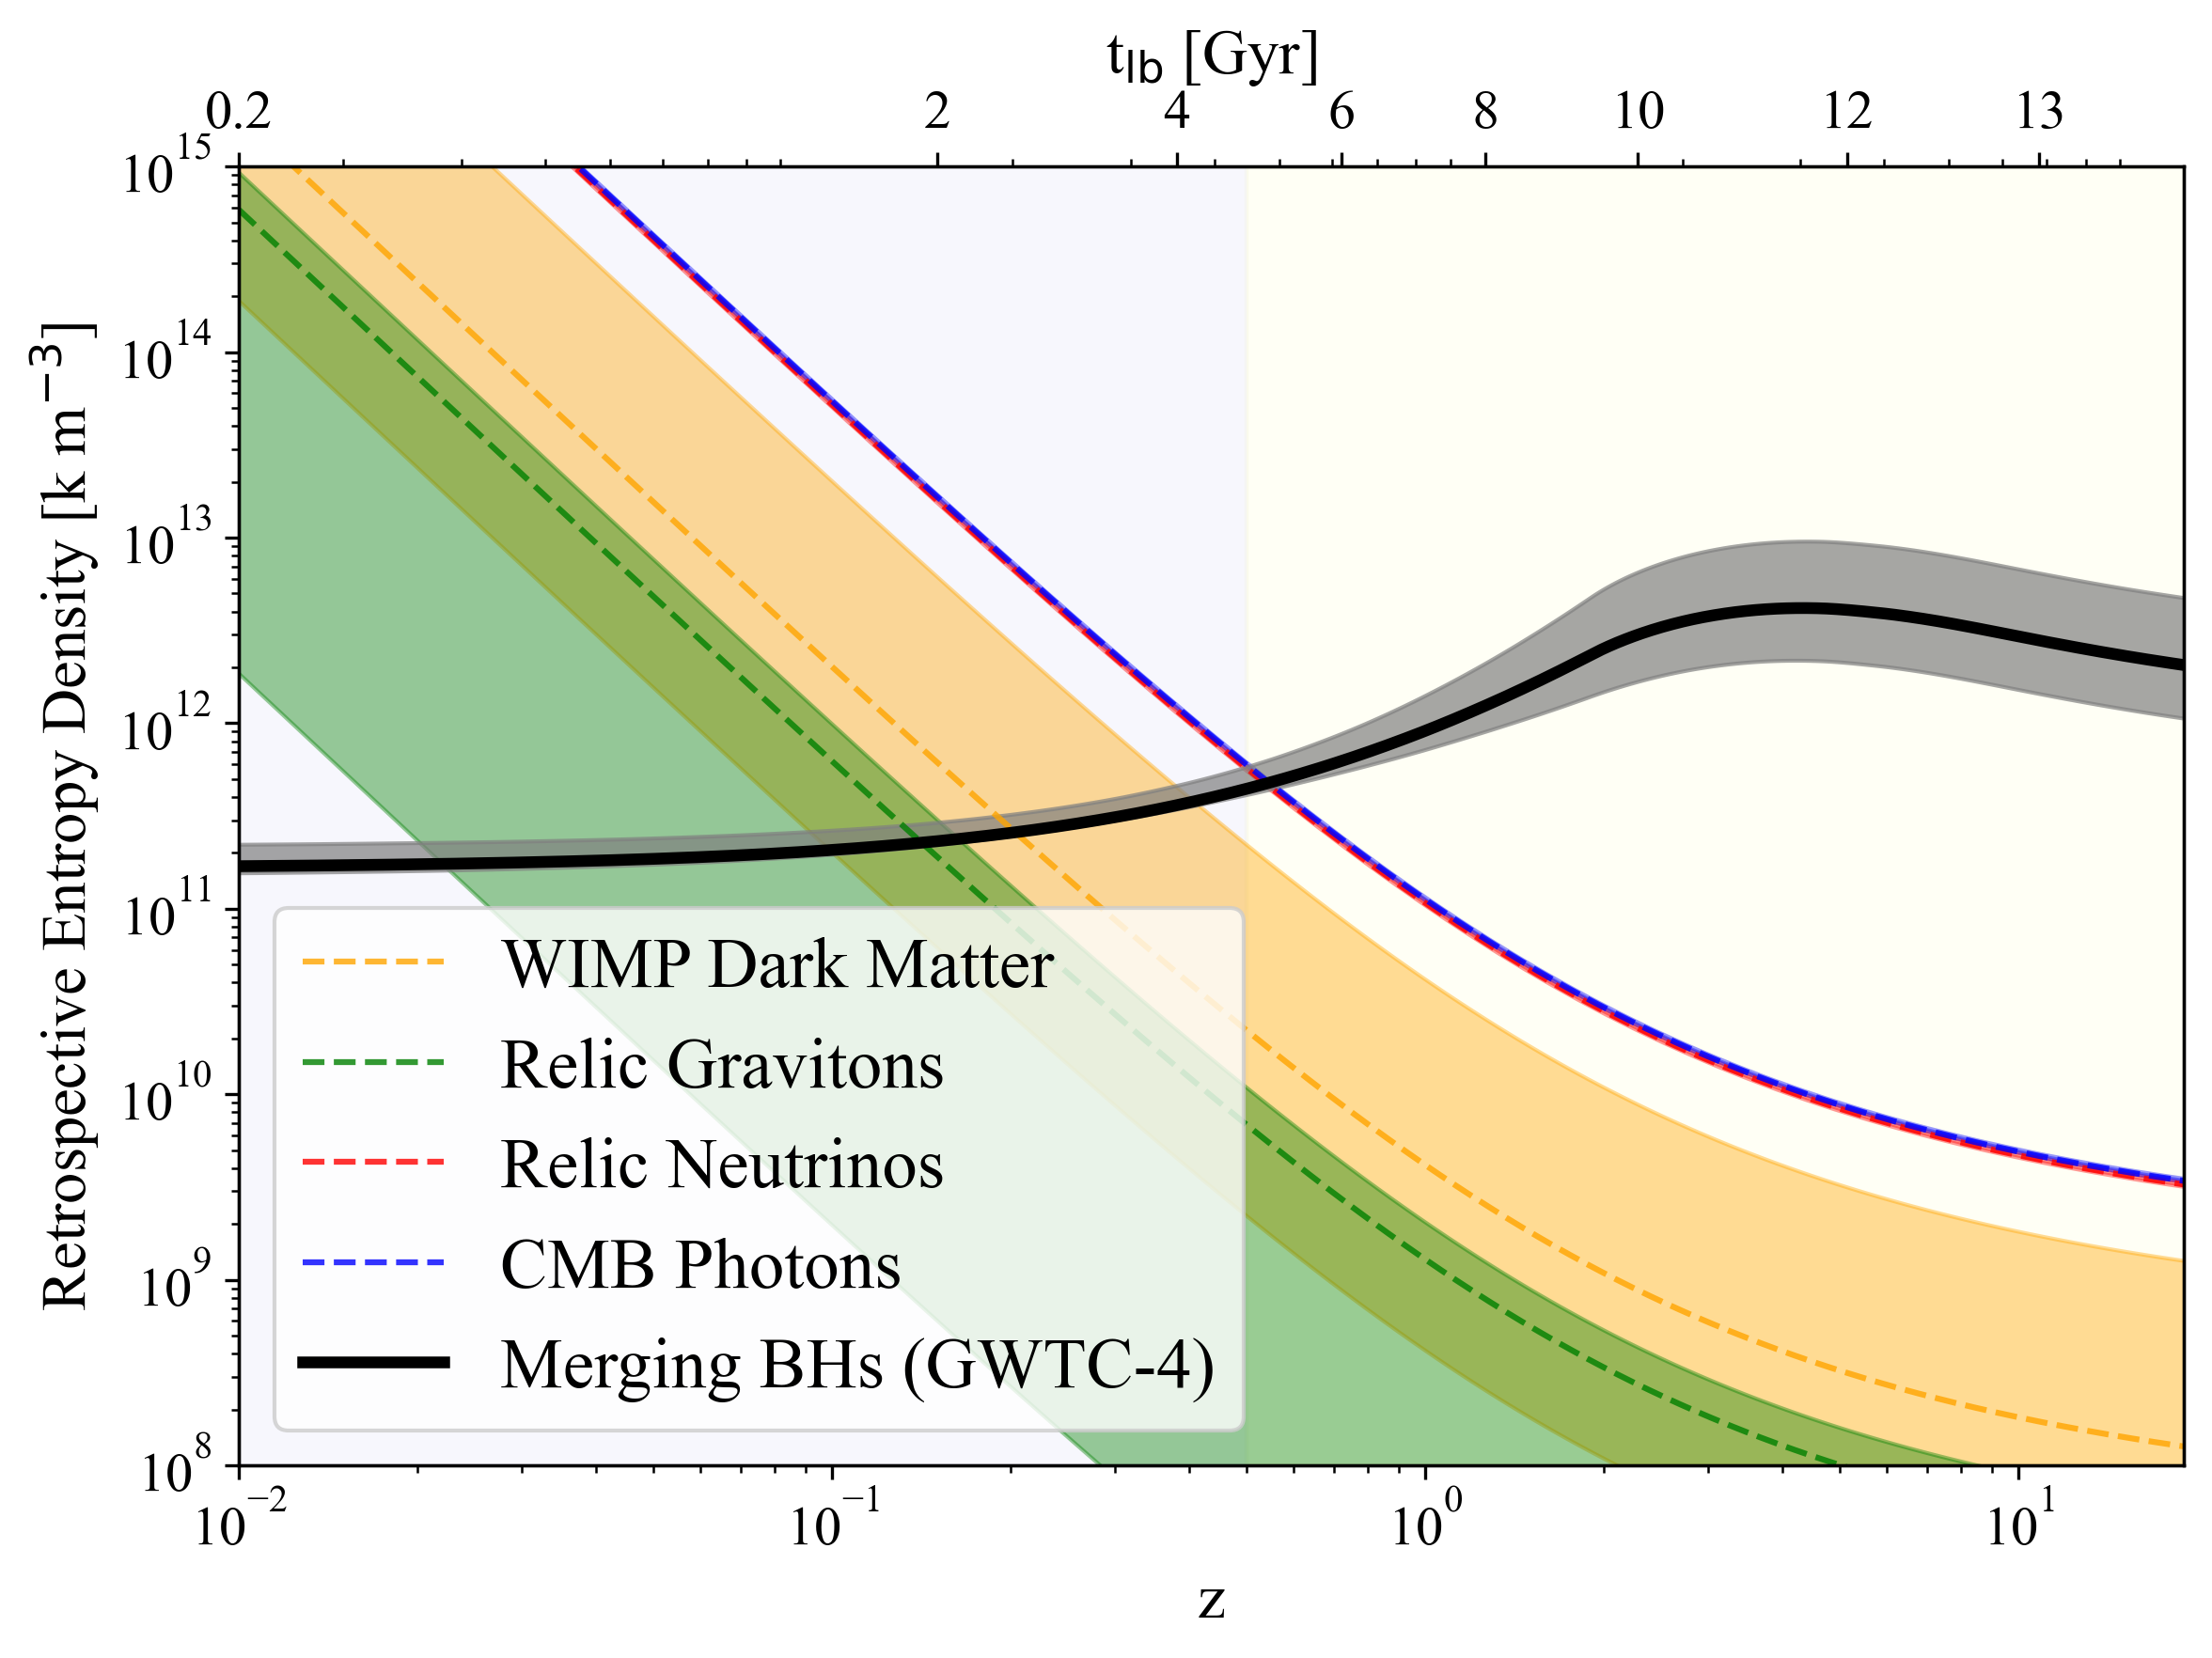
\includegraphics[width=0.49\textwidth]{cumulative_ent_den_gwtc4_only.png}
\caption{\textbf{Volume-normalized Retrospective Entropy Density}: retrospective entropy density as a function of redshift $z$ (bottom x axis) and look-back time $t_{lb}$ (top x axis), constructed by normalizing the cumulative entropy budget integrated over $z\in [0.01,20]$ by the comoving volume enclosed within the same interval. For reference, we include the entropy contributions of several conserved cosmic components reported in \cite{Egan_2010}. The purple-shaded region corresponds to the dark energy–dominated era ($z \le 0.5$), while the yellow-shaded region represents the matter-dominated era ($z > 0.5$).
%The blue curve represents the total growth entropy ($\frac{\Delta S}{\Delta V \Delta t} dt dV$), where we use the BBH merger rate to multiply the differential comoving volume $dV$ and differential lookback time $dt$. The red curve represents the growth entropy density ($\frac{\Delta S}{\Delta V \Delta t}dt$). The scale of total growth entropy and entropy density are shown in the two vertical axes.
\label{fig:rate}
}
\end{figure}

For context, Fig. \ref{fig:rate} shows the profiles of several conserved cosmic components using entropy budgets compiled in \cite{Egan_2010}. For these relic populations, the total entropy budget is approximately conserved following Big Bang Nucleosynthesis, so their retrospective entropy density under Eq. \ref{eq:rate_entropy_density} is obtained by distributing a fixed total entropy over an increasing enclosed comoving volume $V_c(<z_0)$. Consequently, their curves decrease monotonically with increasing $z_0$, with the evolution driven entirely by the comoving volume normalization rather than intrinsic entropy production.

Under this retrospective normalization, the curve for BBH-merger becomes comparable to and intersects the baselines for relic photons and relic neutrinos near $z=0.55^{+0.01}_{-0.05}$, broadly coinciding with the transition between dark energy–dominated and matter-dominated eras. We stress that this intersection should be interpreted strictly within the context of the adopted volume-normalized cumulative definition. It signifies that, when averaged over the local comoving volume enclosed within $z \approx 0.5$, the integrated entropy produced by astrophysical black hole mergers is sufficient to rival the volume-diluted density of relic radiation backgrounds.



% total entropy accumulated over cosmic time, highlighting the contribution of BBH mergers to the cosmological entropy budget from the earliest structure formation epochs to today. Notably, the cumulative entropy produced by BBH mergers increases monotonically with time and eventually exceeds the entropy associated with the cosmic microwave background (CMB) photons at a redshift of $z \sim 12.6^{+1.5}_{-3.5}$.

% The James Webb Space Telescope (JWST) reported the detection of an accreting black hole of $\sim 4 \times 10^7~M_\odot$ in galaxy UHZ1 at $z \sim 10.1$ \citep{natarajan2023detectionovermassiveblackhole}, currently the most distant black hole observed. Theoretical models predict a transient phase of Over-massive Black hole Galaxies (OBGs) between $z \in [9,12]$ \citep{2013MNRAS.432.3438A, Natarajan_2017}, which is also highlighted in the figure.  Intriguingly, the cumulative entropy from BBH mergers is found to exceed that of CMB around the transient OBG stage, suggesting that black hole mergers were already contributing significantly to the thermodynamic state of the universe than the relic radiation from the Big Bang during this early epoch. This result implies that stellar black hole mergers had become a dominant source of entropy production in the infant universe, potentially supporting seeding models in which Population III stars collapse into black hole seeds in the mass range of $10-100~M_\odot$. These seed black holes may merge at $z \ge 12$ and gradually form SMBHs observed by JWST at high redshifts. \scccc{There may be more to write about here - we may discuss? or primordial black holes?}



% We introduce a new variable called \textit{rate entropy} to characterize the ratio between the total entropy and the corresponding comoving volume enclosed within a given redshift $z$:

% \begin{equation}
%     \mathrm{Entropy~Density~Rate~(z)} = \frac{S_{~\in[0,z]}}{V_{c~\in[0,z]}}
% \end{equation}

% In this reference frame,
% we sum up all the entropy increase produced by BBH mergers within $z$. 

% \scccc{\subsection{Cosmological Constants from GW}}
% \scccc{report the results here: $\Omega_\mathrm{BH}$, $\Omega_\mathrm{BH,~rem} = 4.19^{+5.68}_{-2.44} \times 10^{-9}$, $\Omega_\mathrm{GW} = 5.01^{+6.50}_{-2.85} \times 10^{-11}$.}

% \scccc{Connect to CMB photons and neutrinos. $\Omega_\gamma \approx 5 \times 10^{-5}$, $\Omega_\nu \approx 3.4 \times 10^{-5}$, GW is non-thermal radiation. While Black Holes have overtaken the universe in terms of entropy, Energy of photons is much larger than that released from merging BBHs - most mass-energy still retained in the remnant black holes? The merger process is extremely efficient at conserving mass-energy within the event horizon.}

% \scccc{The Thermodynamic Efficiency of Black Hole MergersOur calculation of $\Omega_{GW} \approx 5 \times 10^{-11}$ places the stochastic gravitational-wave background six orders of magnitude below the cosmic microwave background ($\Omega_{\gamma} \sim 10^{-5}$), confirming that while black hole mergers are the dominant source of the universe's entropy, they are a negligible contributor to its energy budget.This dichotomy completes the thermodynamic picture of compact object coalescences. In accordance with the First Law of Thermodynamics, the progenitor mass is conserved, partitioned between the remnant black hole ($\Omega_{BH} \sim 10^{-9}$) and the radiated energy ($\Omega_{GW} \sim 10^{-11}$). In accordance with the Second Law, this small release of energy facilitates a disproportionately large increase in entropy. Thus, we interpret $\Omega_{GW}$ not merely as a background radiation field, but as the necessary energetic by-product of the universe's drive toward its maximum entropy state.}

% We define a new reference frame called rate entropy, which is the ratio between the total entropy within redshift z and the comoving volume within redshift z. We treat Earth as the center of the universe though it’s not true. For example we want to calculate the rate entropy at redshift 1, we sum up all the entropy increase from BBH mergers within this circle and divided by the comoving volume in this circle. Since it is cumulative, both quantities will monotonically increase, and it gives a novel way to see how the two variables balance between each other across redshifts. We also add some other components in the graph assuming their number conserves across the universe. We find that the rate entropy of CMB photons and also relic neutrinos intersect with the rate entropy of merging black holes just at the boundary between the DE and matter-dominated regions

% In the dark energy-dominated era (purple region), the universe expands \textit{exponentially}, at a much faster rate than during the matter-dominated era (yellow region), where expansion follows a \textit{power law} relationship. In Fig. \ref{fig:rate}, we introduce a variable called the entropy density rate ($\frac{S_{\in[0,z]}}{V_{c~\in[0,z]}}$). The entropy density rate at redshift $z$ is computed as the total entropy increase from all BBH mergers \textbf{within $z$} divided by the comoving volume \textbf{within $z$}. The number of BBH mergers within $z$ is obtained from Eq. \ref{eq:cumulative}. This variable allows us to examine the correlation between BBH merger rate and the volume expansion of the universe. 


% Therefore, the growth of entropy is expected to decrease drastically in the dark energy-dominated era (orange), while the decrease should be slower in the matter-dominated era. 







% \subsection{Net Entropy in the Mass-Spin Parameter Space}



% Unlike the mass distribution, there is no similar offset in the spin distribution.



% Unlike mass, spin magnitude does not significantly contribute to . As visualized in Fig. \ref{fig:spin} - although the entropy of a black hole should be largest at $a \sim 0$, there is not an offset similar to the mass distribution. Rather, $\Delta S$ is still the largest at $a \sim 0.2$.



% \subsection{Entropy of Black Holes in the Upper Mass Gap}



% In Fig. \ref{fig:mass}, we show the number density and entropy increase per logarithmic mass interval. The number density and entropy distribution follows the mass distribution from GWTC-3, with the characteristic of double peaks. The number density is maximum at the peak with lower mass, while the entropy increase is maximum at the peak with higher mass. At $M = 34.96~M_\odot$, $\Delta S = 1.98 \times 10^{90}~k$, and at $M = 8.97~M_\odot$, $\Delta S = 1.49 \times 10^{90}~k$. As shown in Eq. \ref{eq:entropy}, entropy of a black hole correlates to $M^2$. Higher mass at the peak of $\sim 35~M_\odot$ offsets with the lower number density.

% The entropy increase contributed by BBHs inside the PISN mass gap constitutes 15\% of the total entropy increase, while the number of BBHs in the PISN mass gap only constitutes 1.5\%.




% $\mathcal{R}(z)$

% Mass distribution from GWTC-3 (PowerLaw + Peak model)

% \scccc{
% \begin{enumerate}
%     \item Entropy of all LIGO events
%     \item Dependence of entropy on the astrophysical distribution of BBH mass and spins
%     \item Entropy production (per year) in the local universe from BBH mergers
%     \item Total entropy and entropy density from all stellar BBH mergers in the universe
%     \item Entropy growth from BBHs across the expansion of the universe from z=20 to z=0
% \end{enumerate}
% }
% need paraphrase, just quote the paper




% In Fig. \ref{fig:lvk}, we illustrate the entropy change during BBH mergers for all 83 confirmed BBH events reported by LVK \citep{gwtc-1, gwtc-2, gwtc-3, gwtc-2.1}. For all events reported by LVK, we utilize the parameter estimation results made available in the GW Open Science Center \citep{2021SoftX..1300658A, 2023ApJS..267...29A}. We use the posteriors from SEOBNRv4PHM waveform \citep{Buonanno_1999, Buonanno_2000, Damour_2008, Ossokine_2020, gadre2022fullyprecessinghighermodesurrogate}. The files also include the mass and spin associated with the corresponding remnant black hole, which has been computed using phenomenological fits to NR results \citep{Santamar_a_2010, Hofmann_2016, Healy_2017, Jim_nez_Forteza_2017,  Estell_s_2022}. We input the posteriors of primary, secondary, and remnant black holes in  Eq. \ref{eq:bh_for} and compute the corresponding change in entropy for each LVK event.




% We plot the entropy change of individual BBH merger in Fig. \ref{fig:lvk}, showing the correlation of entropy change with primary mass and redshift respectively. We highlight several special events, including the most massive BBHs GW190426 \citep{gwtc-2.1} and GW190521 \citep{LIGOScientific:2020iuh, gwtc-2}, the lightest BBH GW190924 \citep{gwtc-2, alfradique2023darksirenmeasurementhubble}, BBH with spin-orbit misalignment GW191109 \citep{gwtc-3, zhang2023likely}, and two stellar-mass BBHs GW190503 and GW190720 for reference.

% From Fig. \ref{fig:lvk}, we observe the expected correlation between mass and entropy indicated in Eq. \ref{eq:bh_for}. The more massive the black hole, the more entropy it increases after the merger. The two most (least) massive BBHs indeed show largest (smallest) change in entropy. The plot shows a linear relationship in the log-log scale, with some outlier events from asymmetric BBHs like GW190403 ($q = 0.25^{+0.54}_{-0.11}$) \citep{Qin_2022} and GW190412 ($q = 0.28^{+0.12}_{-0.06}$) \citep{LIGOScientific:2020stg}. 
% Observing compact object coalescence beyond z $\geq$ 2 can be challenging for current ground-base detectors \citep{Mancarella_2023}, and there is not an explicit relationship between redshift z $\in$ [0,2] and entropy change in the right plot of Fig. \ref{fig:lvk}. However, the highlighted events show some trivial and weak relationship: the higher the redshift, the larger the increase in entropy. Redshift has some correlation with mass \citep{Rinaldi_2024}, favoring high-mass regime when redshift increases. However, in the population analysis, we do not account for this weak correlation, assuming the mass distribution of black holes is independent of redshift. The mass distribution from Power-Law + Peak model is also consistent across the redshift spectrum \citep{KAGRA:2021duu}.



% \subsection{Entropy of Black Hole Population}
% According to the population inferred from GWTC-3 \citep{gwtc-3-pop}, black holes with low spin ($\chi \lesssim 0.25$) constitute the majority of the population. Similarly, there are more mergers for individual black holes of $\sim 10~M_\odot$, as well as a slightly high probability around $\sim 35~M_\odot$, which aligns with the PowerLaw + Peak model. The properties of this model determine the number of BBH mergers that happened within $z \in [0,~20]$. Therefore, the number of BBH mergers depends on the parameter distribution, ultimately impacting the total entropy increase. Therefore, $\Delta S$ across the universe follows the trend of $\frac{dN}{da}$ and $\frac{dR}{dm}$ derived from GWTC-3 population, as shown in Fig. \ref{fig:spin}.










% Similarly, we can calculate $\Delta S$ in mass ($M_\mathrm{tot}$) - redshift (z) parameter space. We assume the mass distribution of BBH is consistent across every redshift. Based on \cite{Mapelli_2018}, the BBH merger rate peaks at $z \sim 2.5$, where the entropy density of BBH mergers is the maximum. When we incorporate comoving volume $V_c$, the total number of mergers peaks at $z \sim 4$ since the differential $V_c$ increases as z increases. We will elaborate more on the scaling shift between entropy and entropy density in Fig. \ref{subsec:cosmo}. The total entropy change from BBH mergers across the parameter space is $\Delta S = 1.3^{+1.6}_{-1.2} \times 10^{92}~k$, $\frac{dS}{dV_c} = 8.1^{+9.6}_{-7.1} \times 10^{11}~k~m^{-3}$, which can be added to Table 1 in \cite{Egan_2010}. With the recent GW detection by LVK, we can update the table for the entropy budget. Events, including GW190426 and GW190521, have proven the existence of stellar black holes within the PISN mass gap ($\sim 42~M_\odot - 140~M_\odot$), where their entropy budget is calculated but listed as tentative in \cite{Egan_2010}. Both the entropy and entropy density from stellar BBH mergers rank fourth in the table, preceded by SMBHs, Stellar BHs ($\sim 42~M_\odot - 140~M_\odot$), and Stellar BHs ($2.5~M_\odot - 15~M_\odot$).


% As shown in Fig. \ref{fig:density}, both $\Delta S$ and $\frac{dS}{dV_c}$ exhibit two peaks at $M_\mathrm{tot} \sim 20~M_\odot$ and $\sim 70~M_\odot$ following PowerLaw + Peak. However, the peaks of $\Delta S$ and $\frac{dS}{dV_c}$ do not occur at the same redshift. The distribution of $\frac{dS}{dV_c}$ scales with the differential comoving volume in the $\Delta S$ distribution.

% \scccc{elaboration on updated table}

% We recreate the entropy budget table for black holes of all mass ranges in  Table \ref{tab:budget}.

%Merging BBHs contribute much smaller total entropy $S$ compared with stellar BHs, while the entropy density is still comparable. Since the first merging BBH is expected to appear at z < 10 after the first star formation \citep{van_Son_2022_1}, the volume will be much smaller than the observable universe.






% \scccc{item 3 - ???}


% entropy density is a scale matter of total entropy here 



% \subsection{BBH Entropy \& Cosmology}
% \label{subsec:cosmo}
% \scccc{item 5 - still need to simulate the plot for this for z against entropy in unit of [Gpc-3yr-1]}

% \scccc{dark matter, matter, radiation-dominated regions plot}





% At $z \sim 2.79$, the merger rate of BBH is maximum, so the entropy growth as this redshift is maximum. At this turning point, the total number of BBH mergers balance out the expansion of the universe. Currently, LVK detector can hardly observe BBH mergers beyond $z \sim 2$, so the GWTC-3 cannot yet observe the balance point at $z \sim 2.79$. The entropy growth in the dark energy-dominated region nearly overlap between the merger rates derived from GWTC-3 and Illustris simulations in \cite{Mapelli_2018}. However, the entropy growth rate from two models diverge in the matter-dominated era. GWTC-3 predicts much more BBH mergers at the matter dominated region, which results in higher entropy growth rate.




% \begin{figure}[hbt!]
% \includegraphics[width=0.5\textwidth]{entropy_tot_ETCE.png}
% \caption{Total increase of entropy at each redshift due to BBH mergers. Two thrid-generation detectors CE \& ET are simulated here.}
% \label{fig:etce}
% \end{figure}

% \begin{figure}[hbt!]
% \includegraphics[width=0.5\textwidth]{entropy-contour.png}
% \caption{Entropy density at each redshift bin of 0.01. The color scheme shows the magnitude of entropy density, and the value is normalized to create the contour.}
% \label{fig:countor}
% \end{figure}

% From GWTC-3 population \citep{Talbot_2018}, we can infer the BBH merger rate in terms of mass and redshift shown in Fig. \ref{fig:redshift}. With the merger rate, we can calculate the total number of BBH mergers in the universe and the total entropy change. GWTC-3 population gives an inferred R(z) function where the merger rate depends on the redshift shown in the top graph in Fig. \ref{fig:redshift}. We use the PowerLawRedshift function from the gwpopulation package to fit the merger rate between z=0 and z=1.5. This small range facilitates our calculation in the local universe. The package estimates R(z=0) $\approx$ 18GPc$^{-3}$yr$^{-1}$ and R(z=1.5) $\approx$ 883GPc$^{-3}$yr$^{-1}$. Therefore, between the two redshifts, there is a scale factor of around 50. As redshift increases, the merger rate monotonically increases as an exponential curve. We expect more BBH events to be observed with higher redshift, so the total entropy change should be larger.

% \begin{figure*}[hbt!]
% \centering
%     \includegraphics[width=0.4\textwidth]{download-85.png}
% \label{fig:redshift}
% \caption{Merger rate function related to redshift R(z) inferred from GWTC-3 population. This function is fitted with the PowerLawRedshift function from the gwpopulation package.}
% \end{figure*}

% \begin{figure*}[hbt!]
% \centering
%     \includegraphics[width=0.4\textwidth]{download-86.png}
% \label{fig:dR/dm}
% \caption{Merger rate function related to mass in differential form $\frac{dR}{dm}$ inferred from GWTC-3 population, which is consistent with the PowerLaw + Peak model.}
% \end{figure*}

% \begin{figure*}[hbt!]
% \centering
%     \includegraphics[width=0.4\textwidth]{download-86.png}
% \label{fig:dR/dm}
% \caption{Merger rate function related to mass in differential form $\frac{dR}{dm}$ inferred from GWTC-3 population, which is consistent with the PowerLaw + Peak model.}
% \end{figure*}


% Another merger rate that GWTC-3 infers depends on mass. However, this merger rate appears in a differential form of $\frac{dR}{dM}$ shown in the bottom plot of Fig. \ref{fig:dR/dm}. When integrating this function across all mass ranges between [2.5, 100]$M_{\odot}$, it gives R(z=0) $\approx$ 18GPc$^{-3}$yr$^{-1}$. The mass distribution is consistent with the PowerLaw + Peak model \citep{Talbot_2018}. More lower-mass BBH mergers are expected, especially black holes with mass less than 20$M_{\odot}$. There is a small peak at around 35$M_{\odot}$. This small peak can come from artifacts and selection effects of LIGO. Stellar evolution and nucleosynthesis theory predicts a mass gap between [50, 130]$M_{\odot}$, where black holes should not be born in this range \citep{Woosley_2021}. No black hole is expected to be inside this gap because of the pair-instability supernovae (PISNe), which disrupts the presupernova star and leaves no compact remnant \citep{Farmer_2019}. The precise bounds of the PISNe mass gap are still uncertain \citep{Fishbach_2020} due to different nuclear reaction rates, evolution in detached binaries, rotation speed, and hyper-Eddington accretion for massive stars \citep{Woosley_2021}. The lower bound is especially uncertain and varies in different papers \citep{Marchant_2020}. With LIGO observations, black holes heavier than 40$M_{\odot}$ should correspond to different formation channels. LIGO tends to detect more events lighter than 40$M_{\odot}$. Even if a black hole is inside the PISNe mass gap, the posterior observed by GW detectors can peak around 35$M_{\odot}$. As a result, the merger rate $\frac{dR}{dm}$ is higher at masses slightly lower than 40$M_{\odot}$.



% \begin{figure*}[hbt!]
% \centering
% \includegraphics[width=0.7\textwidth]{merger_rate.jpg}
% \caption{}
% \label{fig:mass}
% \end{figure*}



% From the observed GW events from GWTC-2 \citep{gwtc-2} and GWTC-3 \citep{gwtc-3}, we calculate the entropy change $\Delta S$ for each event shown in Fig. \ref{fig:entropy}. We can see that the values span a very large range. Entropy change can largely vary between different GW events, ranging from 10$^{62}$ to 10$^{66}$. This large range is because the entropy of black holes correlates with mass, as demonstrated in eq. \ref{eq:bh_for} as well. The entropy change of GW190521 (the heaviest BBH merger event) is more than 1000 times larger than GW190924, the confirmed least massive BBH merger. Therefore, if we want to sample from the LIGO population, we will need numerous data points to ensure accuracy.

% Assuming the merger rate is independent of mass (so the overall merger rate is the same as zppd in eq. \ref{eq:merger}), we investigate how the entropy density changes as redshift increases. We use a redshift bin of z=0.3. We have a distribution showing a monotonic increase, shown in Fig. \ref{fig:density}. Total entropy change will increase as redshift increase, so the entropy density will also increase. The order of magnitude for the entropy density is similar to the stellar BHs shown in the entropy budget from \cite{Egan_2010}. Therefore, entropy change from BBH mergers can largely contribute to the universe.

% \begin{figure*}[hbt!]
% \centering
% \includegraphics[width=0.7\textwidth]{download-97.png}
% \caption{Plots of entropy change density and redshift.}
% \label{fig:density}
% \end{figure*}


% As suggested before and shown in Fig. \ref{fig:dR/dm}, BBHs with different masses will correspond to different merger rates. They will have large effects on the calculation of total entropy change. We have to account for the effect of $\frac{dR}{dm}$. We have to change eq. \ref{eq:merger} so that zppd will not be the only dominant term in the total number of BBH mergers N.

% To figure out a merger rate function associated with mass R(m), we can integrate the differential expression between $m-\delta m$ and $m+\delta m$:

% \begin{equation}
% \centering
%     R(m) = \int_{m-\delta m}^{m+\delta m} \ddfrac{dR}{dm} dm
% \end{equation}

% With the R(m) function, we can figure out the total number of BBH mergers we expect to see with specific mass:

% \begin{equation}
% \centering
%     N(m) = \int \ddfrac{dV_c(m)_{det}}{V_c(m)_{O3}} R(m) <VT(m)>_{O3} dz
% \label{eq:det}
% \end{equation}

% where $V_c(m)_{O3}$ is the comoving volume range during the LIGO's 3rd observing run, and $V_c(m)_{det}$ characterizes the detector. VT(m) denotes the sensitive 4-volume for a specific binary. With the $<>$ operator, the volume is averaged over the specific mass range (typically neutron stars with mass less than 2.5$M_\odot$) \citep{KAGRA:2021duu}. VT will be specific to the 3rd observing run because the merger rate comes from simulated sources to a GWTC-3 astrophysical population with a specific hyperparameter. Since we are calculating the total number of BBH mergers with a specific mass, the formula will integrate across all redshifts. 

% In this study, we are not working with a specific GW detector. Therefore, we will substitute the $V_c(m)_{det}$ term in eq. \ref{eq:det}. To calculate the total number of BBH mergers at a specific redshift (less than 1.5), we change the formula as:

% \begin{equation}
% \centering
%     N(m) = \int \ddfrac{dV_c(m)_{z<1.5}}{V_c(m)_{O3}} R(m) <VT(m)>_{O3} dz
% \end{equation}

% However, there is a hidden dependence on redshift in the expression R(m). When the lower and upper bounds $m-\delta m$ and $m+\delta m$ span the whole range of [2.5, 100]$M_{\odot}$, R(m) is same as R(z=0). We need to scale the mass merger rate function with redshift to obtain the total entropy calculation. In future work, we plan to resolve the intricate relationships between redshift and source mass to figure out the total number of BBH mergers in the universe.

% \scccc{Leave the conclusion parts first}

\section{Conclusion}
In this study, we have presented a revised cosmic entropy budget, explicitly quantifying the contributions from stellar-collapse black holes and their mergers. By integrating LVK event-level posteriors with GWTC-3/4 population inference and cosmological merger rate histories, we constructed an inventory driven primarily by the mass spectrum—a direct consequence of the $S \propto M^2$ scaling inherent to the Hawking area theorem. Utilizing the GWTC-4 parameter space, we characterized the dependence of entropy production on mass, spin, and redshift, revealing three key insights. First, we identified a critical "thermodynamic crossover" during Cosmic Dawn ($z \sim 12$). This epoch, coinciding with the predicted OBG phase, marks the moment when the cumulative entropy generated by BBH mergers surpasses the entropic content of the CMB photon background. Second, we demonstrated that even a trace population of primordial black holes would establish an early "entropy floor," dominating the thermodynamic landscape of the Dark Ages. Finally, by computing the cosmological density parameters, we highlighted a profound thermodynamic asymmetry: while BBH mergers are energetically inefficient, radiating only a minute fraction of their mass-energy as gravitational waves, they drive a disproportionate irreversible increase in cosmic entropy.

We acknowledge that our high-redshift conclusions rely on extrapolating the BBH merger rate from \cite{Mapelli_2018} beyond the horizon of current ground-based detectors, leaving $\mathcal{R}(z)$ less constrained at $z\gtrsim2$. Future GW facilities will provide the necessary empirical anchor to test these predictions. Space-based observatories like LISA~\cite{LISAstudyreport} will access lower-frequency signals from massive and IMBH systems out to high redshifts \citep{Rosado_2016, Ng_2022, Mancarella_2023, Wu_2024}, while proposed mid-band concepts such as the Laser Interferometer Lunar Antenna (LILA) would bridge the gap between LVK and LISA, extending sensitivity to heavier binaries and earlier cosmic times \citep{jani_2021, jani2025laserinterferometerlunarantenna, LILAPioneer, LILAHorizon}. Together, these missions will directly map $\mathcal{R}(z)$ over a broader mass range, reducing reliance on star formation rate-based extrapolations and enabling a precise reconstruction of entropy production in the Universe's earliest epochs.


% We compute the entropy budget of different black hole populations, including those associated with the PISN mass gap and IMBHs, which have been previously overlooked. The key findings of our analysis are summarized below:
% \begin{enumerate}
%     \item We compute the entropy budget of stellar black holes and light IMBHs formed from VMSs. Our results are consistent with previous estimates.
%     \item We populate the PISN mass gap with merging black holes and find that their total entropy contribution is approximately $10^7$ times less than that of other black hole populations. This highlights the limited formation pathways for black holes in the PISN regime and underscores the thermodynamic distinctiveness of this mass range.
%     \item We demonstrate that entropy growth in the dark energy–dominated era follows a power-law behavior, governed by the interplay between cosmic volume expansion and the BBH merger rate.
%     \item We derive a new variable called \textit{Entropy Density Rate} \scccc{more cosmology}
% \end{enumerate}
% After connecting entropy with GWs with the Hawking Area Theorem, we investigated how much entropy BBH mergers contributed to the universe. We first computed the entropy change for all individual GW events reported by LIGO, showing large variations between black holes. Heavier black holes will radiate more entropy to the spacetime during the merger. We adopted the inferred GWTC-3 populations and figured out the post-merger conditions with numerical relativity fit, which also corrected the selection effects of GW detectors. With the merger rate derived from LIGO populations, we could calculate the total number of BBH mergers at certain redshifts, thus measuring the total entropy change. We showcase that as redshift increases, the total entropy change and the entropy density will monotonically increase, with an order of magnitude aligned with stellar-mass black holes. To ensure a more accurate measurement that accounts for every parameter, we plan to figure out the intricate relationships between mass and redshift in merger rate calculations in the future. 

\section{Acknowledgement}
We thank Priyamvada Natarajan for insightful discussion. S.C. acknowledges the support from the Littlejohn Fellowship, Vanderbilt Immersion Program and the Vanderbilt University Summer Research program. K. J.’s work was supported in part by the Lunar Labs Initiative at Vanderbilt
University, which is funded by grants from the John Templeton Foundation and the Vanderbilt Scaling Grant from the Office of the Vice Provost for Research and Innovation. This material is based upon work supported by NSF’s LIGO Laboratory, which is a major facility fully funded by the National Science Foundation. This research has made use of data, software and / or web tools obtained from the Gravitational Wave Open Science Center (\url{https://www.gw-openscience.org/}), a service of LIGO Laboratory, the LIGO Scientific Collaboration and the Virgo Collaboration. LIGO Laboratory and Advanced LIGO are funded by the United States National Science Foundation (NSF) as well as the Science and Technology Facilities Council (STFC) of the United Kingdom, the Max-Planck-Society (MPS), and the State of Niedersachsen/Germany for support of the construction of Advanced LIGO and construction and operation of the GEO600 detector. Additional support for Advanced LIGO was provided by the Australian Research Council. Virgo is funded, through the European Gravitational Observatory (EGO), the French Centre National de Recherche Scientifique (CNRS), the Italian Istituto Nazionale di Fisica Nucleare (INFN), and the Dutch Nikhef, with contributions by institutions from Belgium, Germany, Greece, Hungary, Ireland, Japan, Monaco, Poland, Portugal, Spain.

% \bibliographystyle{plain} 
\bibliography{sample631}

\end{document}

% End of file `sample631.tex'.
